\hypertarget{group__dcsc__msg__buffer__access}{
\section{Message Buffer Encoding}
\label{group__dcsc__msg__buffer__access}\index{Message Buffer Encoding@{Message Buffer Encoding}}
}
This module implements the basic access function to DCS board message\_\-buffer\_\-interface via the \hyperlink{group__rcubus__driver}{RCU bus driver}.  
\subsection*{Message Buffer Header Format Version.}
Version handling has been introduced in firmware version 2.

\small\begin{alltt}
 Bit 28-31 of message buffer header
 0x0     : not used
 0x1-0x7 : version 1 (bit 31==0, other bits arbitrary)
 0xa     : version 2
 0xf     : Feeserver CE command
 \end{alltt}\normalsize 


{\bf Some helper defines} for the version decoding: \begin{CompactItemize}
\item 
\#define \hyperlink{group__dcsc__msg__buffer__access_gd47e658eba41557f654f0f9284c97317}{MSGBUF\_\-VERSION\_\-1\_\-MASK}~0x70000000
\begin{CompactList}\small\item\em Mask to extract Message Buffer Version 1 command ids. \item\end{CompactList}\item 
\#define \hyperlink{group__dcsc__msg__buffer__access_g4fc7f5db2448d65028809260a6d7879f}{MSGBUF\_\-VERSION\_\-2}~0xa0000000
\begin{CompactList}\small\item\em Message Buffer Version 2.0 id. \item\end{CompactList}\item 
\#define \hyperlink{group__dcsc__msg__buffer__access_gbe9b5c0065d5ca89ab3c3af7723c5340}{MSGBUF\_\-VERSION\_\-2\_\-2}~0xb0000000
\begin{CompactList}\small\item\em Message Buffer Version 2.2 id. \item\end{CompactList}\item 
\#define \hyperlink{group__dcsc__msg__buffer__access_g4922cdfb6125eef890c22cadeb1a4522}{FEESERVER\_\-CMD}~0xf0000000
\begin{CompactList}\small\item\em Fee\-Server command id. \item\end{CompactList}\end{CompactItemize}
\subsection*{Format of the command result (32 bit words).}
The result given in the MRB has the format:

\small\begin{alltt}
 ============================================
 1.information word (same format as above)
 2.status word
 3.- n: the data words follow
 Bit 0-15 of the information word contain the number of words in the buffer
          including status and information word. There is no end marker\end{alltt}\normalsize 


\small\begin{alltt} Status word: = 0 if no error
 Bit 15: set if any error
 \end{alltt}\normalsize 
 The interface uses the following defines to interprete the error bits: \begin{CompactItemize}
\item 
\#define \hyperlink{group__dcsc__msg__buffer__access_g08c36f682621c241c61818a20deb25c1}{MSGBUF\_\-STATUS\_\-NOMARKER}~0x01
\begin{CompactList}\small\item\em Status Word Bit 0: missing marker. \item\end{CompactList}\item 
\#define \hyperlink{group__dcsc__msg__buffer__access_gc30e76b52c140c354f56d34019c7f1d2}{MSGBUF\_\-STATUS\_\-NOENDMRK}~0x02
\begin{CompactList}\small\item\em Status Word Bit 1: missing end marker. \item\end{CompactList}\item 
\#define \hyperlink{group__dcsc__msg__buffer__access_g4eee888217162b8a35eb12d67cb4693b}{MSGBUF\_\-STATUS\_\-NOTGTASW}~0x04
\begin{CompactList}\small\item\em Status Word Bit 2: no target answer (something wrong with the RCU or not connected). \item\end{CompactList}\item 
\#define \hyperlink{group__dcsc__msg__buffer__access_g2c69c8f183428cc8448002ccbb40223f}{MSGBUF\_\-STATUS\_\-NOBUSGRT}~0x08
\begin{CompactList}\small\item\em Status Word Bit 3: no bus grant (no access to the bus on dcs board). \item\end{CompactList}\item 
\#define \hyperlink{group__dcsc__msg__buffer__access_g63adfcc12380aecaee776059a90bae31}{MSGBUF\_\-STATUS\_\-OLDFORMAT}~0X10
\begin{CompactList}\small\item\em Status Word Bit 5: old message buffer format (prior to v2 with rcu-sh version v1.0). \item\end{CompactList}\end{CompactItemize}
\subsection*{API methods: Initialization and general methods.}
\begin{CompactItemize}
\item 
\#define \hyperlink{group__dcsc__msg__buffer__access_gce40b0def5fb1f60ecebe3d5c07dceb5}{DCSC\_\-INIT\_\-FORCE\_\-V1}~0x0001
\begin{CompactList}\small\item\em Initialization flag: force message buffer format version v1 This sets the encoding to version 1 fixed rather than trying to get the correct firmware version. \item\end{CompactList}\item 
\#define \hyperlink{group__dcsc__msg__buffer__access_g24923a207203a43bfd322e7116edf028}{DCSC\_\-INIT\_\-FORCE\_\-V2}~0x0002
\begin{CompactList}\small\item\em Initialization flag: force message buffer format version v2. \item\end{CompactList}\item 
\#define \hyperlink{group__dcsc__msg__buffer__access_g1283f28b3ca2f03f4cfef9a0f8a8ce40}{DCSC\_\-INIT\_\-ENCODE}~0x0100
\begin{CompactList}\small\item\em Initialization flag: write block to device/file but do not execute. \item\end{CompactList}\item 
\#define \hyperlink{group__dcsc__msg__buffer__access_g1bf79fbd2d8c4bcfbed37007a5e9d4b0}{DCSC\_\-INIT\_\-APPEND}~0x0200
\begin{CompactList}\small\item\em Initialization flag: Append to file. \item\end{CompactList}\item 
\#define \hyperlink{group__dcsc__msg__buffer__access_g3a969c22c4b8fc27c201023112f70bb7}{DCSC\_\-SUPPR\_\-STDERR}~0x0400
\begin{CompactList}\small\item\em Initialization flag: suppress stderr output. \item\end{CompactList}\item 
\#define \hyperlink{group__dcsc__msg__buffer__access_g1d0799f8bf0c0b77db6155e5d78a4619}{DCSC\_\-SKIP\_\-DRV\_\-ADPT}~0x1000
\begin{CompactList}\small\item\em Initialization flag: skip automatic adaption to driver properties. \item\end{CompactList}\item 
typedef \hyperlink{structdcscInitArguments__t}{dcsc\-Init\-Arguments\_\-t} \hyperlink{group__dcsc__msg__buffer__access_gc35123ecbeaf4345c7ea161d1d31b500}{Tdcsc\-Init\-Arguments}
\begin{CompactList}\small\item\em Type definition for extended initialization parameters. \item\end{CompactList}\item 
int \hyperlink{group__dcsc__msg__buffer__access_gfc4448a8f5f9654cf54ad494f1558594}{init\-Rcu\-Access} (const char $\ast$p\-Device\-Name)
\begin{CompactList}\small\item\em Initialize the interface. \item\end{CompactList}\item 
int \hyperlink{group__dcsc__msg__buffer__access_g95f13464dd4da9231a53e7adbb0e7d4e}{init\-Rcu\-Access\-Ext} (const char $\ast$p\-Device\-Name, \hyperlink{structdcscInitArguments__t}{Tdcsc\-Init\-Arguments} $\ast$p\-Arg)
\begin{CompactList}\small\item\em Extended initialization. \item\end{CompactList}\item 
int \hyperlink{group__dcsc__msg__buffer__access_gac62a9e57c67af4cb9178b4426ec12fb}{release\-Rcu\-Access} ()
\begin{CompactList}\small\item\em Close the device and release internal data structures. \item\end{CompactList}\item 
void \hyperlink{group__dcsc__msg__buffer__access_g919bc832f5a0e82c07cfafd699b1b2ea}{print\-Driver\-Info} (int i\-Verbosity)
\begin{CompactList}\small\item\em Get driver info from the driver and print it. \item\end{CompactList}\item 
void \hyperlink{group__dcsc__msg__buffer__access_g0adb3aacb8d7ad32ceabe66a9dcbb401}{start\-Simulation} ()
\begin{CompactList}\small\item\em Start register simulation. \item\end{CompactList}\item 
void \hyperlink{group__dcsc__msg__buffer__access_gd871881385919aff64a8b679984cd018}{stop\-Simulation} ()
\begin{CompactList}\small\item\em Stop the simulation. \item\end{CompactList}\item 
void \hyperlink{group__dcsc__msg__buffer__access_gb54d216419ff2c191363373bef5f9cfa}{reset\-Simulation} ()
\begin{CompactList}\small\item\em Reset the simulation. \item\end{CompactList}\end{CompactItemize}
\subsection*{Interface debug options}
The debug output of the interface can be adjusted by a couple of flags. Flags can be changed by the \hyperlink{group__dcsc__msg__buffer__access_g36bb01dae6dd6edf579fe9878f9c6a20}{set\-Debug\-Option\-Flag}, \hyperlink{group__dcsc__msg__buffer__access_g41201fc4dd5608bce4261b34eec28ca4}{clear\-Debug\-Option\-Flag} and \hyperlink{group__dcsc__msg__buffer__access_gc07186b103fbe4c39531665c95e22c7e}{set\-Debug\-Options} functions. \begin{CompactItemize}
\item 
\#define \hyperlink{group__dcsc__msg__buffer__access_gdcd41743796fdb5a280fc3914121eb05}{PRINT\_\-COMMAND\_\-BUFFER}~0x01
\begin{CompactList}\small\item\em Print the command buffer before writing to the MIB. \item\end{CompactList}\item 
\#define \hyperlink{group__dcsc__msg__buffer__access_gcbc0bfb0d39b96550d664a58aa705cbb}{PRINT\_\-RESULT\_\-BUFFER}~0x02
\begin{CompactList}\small\item\em Print the MRB after executing the command. \item\end{CompactList}\item 
\#define \hyperlink{group__dcsc__msg__buffer__access_g9eba95d21cfe8d57e7d52cadc13e1b91}{CHECK\_\-COMMAND\_\-BUFFER}~0x04
\begin{CompactList}\small\item\em Test the MIB after writing the command buffer to it. \item\end{CompactList}\item 
\#define \hyperlink{group__dcsc__msg__buffer__access_g4115ae88155913f9a07bfbbd995f5e4f}{IGNORE\_\-BUFFER\_\-CHECK}~0x08
\begin{CompactList}\small\item\em Ignore the result of the MIB read back and check. \item\end{CompactList}\item 
\#define \hyperlink{group__dcsc__msg__buffer__access_gc3ceb106888209dd1796a27d49f567d8}{PRINT\_\-REGISTER\_\-ACCESS}~0x10
\begin{CompactList}\small\item\em Print access to the control registers. \item\end{CompactList}\item 
\#define \hyperlink{group__dcsc__msg__buffer__access_g2f996fd7aaf5d3df34642fc4dcd9ef66}{PRINT\_\-COMMAND\_\-RESULT}~0x20
\begin{CompactList}\small\item\em Print the result of the command. \item\end{CompactList}\item 
\#define \hyperlink{group__dcsc__msg__buffer__access_g36c838823c9602c6a0f6efd1fe135b18}{PRINT\_\-SPLIT\_\-DEBUG}~0x40
\begin{CompactList}\small\item\em Print split info for multiple operations. \item\end{CompactList}\item 
\#define \hyperlink{group__dcsc__msg__buffer__access_g6fe994d64da543fe875682bb79b5d585}{DBG\_\-FILE\_\-CONVERT}~0x80
\begin{CompactList}\small\item\em Print debug information on the file conversion. \item\end{CompactList}\item 
\#define \hyperlink{group__dcsc__msg__buffer__access_g5d966eba98a480141a4145615ca3ea15}{PRINT\_\-RESULT\_\-HUMAN\_\-READABLE}~0x100
\begin{CompactList}\small\item\em Print the status bits human readable. \item\end{CompactList}\item 
\#define \hyperlink{group__dcsc__msg__buffer__access_g7eaf88fd984d7f7c8c760dce4cb355d1}{DBG\_\-CHECK\_\-COMMAND}~0x400
\begin{CompactList}\small\item\em Print debug information concerning the wait ('check') command. \item\end{CompactList}\item 
\#define \hyperlink{group__dcsc__msg__buffer__access_gf34c3c30400c83a97dd0deadaead479c}{DBG\_\-DEFAULT}~PRINT\_\-RESULT\_\-HUMAN\_\-READABLE
\begin{CompactList}\small\item\em The default debug flags. \item\end{CompactList}\end{CompactItemize}
\subsection*{Interface error codes.}
The interface uses in general the error codes in errno.h. In addition to that a few more are defined which reflect the error returned in the MRB status word. \begin{CompactItemize}
\item 
\#define \hyperlink{group__dcsc__msg__buffer__access_g2a64137d0941a60d8a7c65c60cf270d1}{EMISS\_\-MARKER}~0x1001
\begin{CompactList}\small\item\em Error indicates a missing marker in the message buffer command. \item\end{CompactList}\item 
\#define \hyperlink{group__dcsc__msg__buffer__access_g0003c432c9b704625105bb7fda5e875e}{EMISS\_\-ENDMARKER}~0x1002
\begin{CompactList}\small\item\em Error indicates a missing end marker at the and of the message buffer command block. \item\end{CompactList}\item 
\#define \hyperlink{group__dcsc__msg__buffer__access_g784f97ba20855df7fdcfb165ba30ba4c}{ENOTARGET}~0x1003
\begin{CompactList}\small\item\em Error in the communication between DCS board and RCU motherboard, no target answer. \item\end{CompactList}\item 
\#define \hyperlink{group__dcsc__msg__buffer__access_g6a6e1cfe5a616e5424852a4519bd47a9}{ENOBUSGRANT}~0x1004
\begin{CompactList}\small\item\em Error on the DCS board internally, no bus grant. \item\end{CompactList}\item 
\#define \hyperlink{group__dcsc__msg__buffer__access_g78f0a660b0b99a94de586d9174999492}{EOLDFORMAT}~0x1005
\begin{CompactList}\small\item\em Error indicates an old message buffer v1 format. \item\end{CompactList}\end{CompactItemize}
\subsection*{Read/write access}
\begin{CompactItemize}
\item 
enum \{ \par
\hyperlink{group__dcsc__msg__buffer__access_gg0411cd49bb5b71852cecd93bcbf0ca2d369f66006fcdc9be0ebe0e56d0dce6c9}{e\-Unknown\-Spec} =  0, 
\hyperlink{group__dcsc__msg__buffer__access_gg0411cd49bb5b71852cecd93bcbf0ca2d1d0f8ecdb452c7ff543d75a98c9cc6b4}{e\-Version}, 
\hyperlink{group__dcsc__msg__buffer__access_gg0411cd49bb5b71852cecd93bcbf0ca2d203d36b00bb0c66542bfbb41283bca1f}{e\-Command}, 
\hyperlink{group__dcsc__msg__buffer__access_gg0411cd49bb5b71852cecd93bcbf0ca2d5c578774a774b0e23c176c8a045b742b}{e\-Nof\-Words}, 
\par
\hyperlink{group__dcsc__msg__buffer__access_gg0411cd49bb5b71852cecd93bcbf0ca2d6678ba12b9d3d2b765aa92a0d12bc1b7}{e\-Packed}
 \}
\begin{CompactList}\small\item\em Operation specifier for the \hyperlink{group__dcsc__msg__buffer__access_g975e68b162a4d0786e1902c895349b02}{dcsc\-Get\-Header\-Attribute} function. \item\end{CompactList}\item 
int \hyperlink{group__dcsc__msg__buffer__access_g5b2ecab6b0a6383afebde1ea486dae43}{rcu\-Single\-Write} (\_\-\_\-u32 address, \_\-\_\-u32 data)
\begin{CompactList}\small\item\em Write a single location (32bit word). \item\end{CompactList}\item 
int \hyperlink{group__dcsc__msg__buffer__access_g339b5922513d0f0211d7962234faa24f}{rcu\-Single\-Read} (\_\-\_\-u32 address, \_\-\_\-u32 $\ast$p\-Data)
\begin{CompactList}\small\item\em Read a single location (32bit word). \item\end{CompactList}\item 
int \hyperlink{group__dcsc__msg__buffer__access_ge20afbfc92c897546e37126188804309}{rcu\-Multiple\-Write} (\_\-\_\-u32 address, \_\-\_\-u32 $\ast$p\-Data, int i\-Size, int i\-Data\-Size)
\begin{CompactList}\small\item\em Write a number of 32bit words beginning at a location. \item\end{CompactList}\item 
int \hyperlink{group__dcsc__msg__buffer__access_g602216accce6913989f8b04b36157cd6}{rcu\-Multiple\-Read} (\_\-\_\-u32 address, int i\-Size, \_\-\_\-u32 $\ast$p\-Data)
\begin{CompactList}\small\item\em Read a number of 32bit words beginning at a location. \item\end{CompactList}\item 
int \hyperlink{group__dcsc__msg__buffer__access_gf7be7371f7530e8eb6e07e6f0d969b04}{dcsc\-Provide\-Message\-Buffer} (\_\-\_\-u32 $\ast$$\ast$pp\-Buffer, int $\ast$p\-Size)
\begin{CompactList}\small\item\em Provide the message buffer for direct access. \item\end{CompactList}\item 
int \hyperlink{group__dcsc__msg__buffer__access_g4f25fcb80c8fad99d5d72f96e72bd941}{dcsc\-Prepare\-Message\-Buffer} (\_\-\_\-u32 $\ast$$\ast$pp\-Buffer, int $\ast$p\-Size, unsigned int cmd\-ID, unsigned int flags)
\begin{CompactList}\small\item\em Prepare the message buffer for a specific command. \item\end{CompactList}\item 
int \hyperlink{group__dcsc__msg__buffer__access_g96f1fe73877d927a698a396df555767e}{dcsc\-Execute\-Command} (\_\-\_\-u32 $\ast$\hyperlink{dcscMsgBufferInterface_8c_7fe69f55846ac3a138c130665f1f1e49}{p\-Buffer}, int i\-Size, \_\-\_\-u32 $\ast$$\ast$pp\-Target, int $\ast$pp\-Target\-Size, unsigned int operation)
\begin{CompactList}\small\item\em Execute the message buffer command. \item\end{CompactList}\item 
int \hyperlink{group__dcsc__msg__buffer__access_g975e68b162a4d0786e1902c895349b02}{dcsc\-Get\-Header\-Attribute} (\_\-\_\-u32 \hyperlink{virtex__io_8h_f662138894a99f1d07d07f482b7c2691}{header}, int i\-Specifier)
\begin{CompactList}\small\item\em Extract a part of the header word according to the specifier. \item\end{CompactList}\item 
int \hyperlink{group__dcsc__msg__buffer__access_g8dac87332689e82a586ef04eed99d083}{dcsc\-Check\-Msg\-Block} (\_\-\_\-u32 $\ast$\hyperlink{dcscMsgBufferInterface_8c_7fe69f55846ac3a138c130665f1f1e49}{p\-Buffer}, int i\-Size, int i\-Verbosity)
\begin{CompactList}\small\item\em Check a message block for correct format. \item\end{CompactList}\end{CompactItemize}
\subsection*{Driver control functions}
\begin{CompactItemize}
\item 
enum \{ \par
\hyperlink{group__dcsc__msg__buffer__access_ggbed82baf7f470b522273a3e37c24c600da3c950575dcbbc7ca50d76a111d217d}{e\-Unknown\-Driver\-Cmd} = 0, 
\hyperlink{group__dcsc__msg__buffer__access_ggbed82baf7f470b522273a3e37c24c600c0b7933997697a647dbfb83d828142f3}{e\-Lock}, 
\hyperlink{group__dcsc__msg__buffer__access_ggbed82baf7f470b522273a3e37c24c600fc021c4ba87bb9763ec7f4e07855d8f9}{e\-Unlock}, 
\hyperlink{group__dcsc__msg__buffer__access_ggbed82baf7f470b522273a3e37c24c6001391714f3c5c8e7738e9b0e871dc3cce}{e\-Seize}, 
\par
\hyperlink{group__dcsc__msg__buffer__access_ggbed82baf7f470b522273a3e37c24c6001349887513e044eb25dceda6bc2c9429}{e\-Release}, 
\hyperlink{group__dcsc__msg__buffer__access_ggbed82baf7f470b522273a3e37c24c600be8853084b74223aab7a0a0c8150eb5a}{e\-Deactivate\-Lock}, 
\hyperlink{group__dcsc__msg__buffer__access_ggbed82baf7f470b522273a3e37c24c60052e15b8bac21d0241661e3caf289e745}{e\-Activate\-Lock}
 \}
\begin{CompactList}\small\item\em Operation ids for the \hyperlink{group__dcsc__msg__buffer__access_gb01774a452cb68f631a87d2d77ac79a5}{dcsc\-Lock\-Ctrl} function. \item\end{CompactList}\item 
int \hyperlink{group__dcsc__msg__buffer__access_gb01774a452cb68f631a87d2d77ac79a5}{dcsc\-Lock\-Ctrl} (int cmd)
\begin{CompactList}\small\item\em Lock the driver. \item\end{CompactList}\item 
int \hyperlink{group__dcsc__msg__buffer__access_g8dc96e96fb45e86a27c98fbe8d816edf}{dcsc\-Driver\-Debug} (unsigned int flags)
\begin{CompactList}\small\item\em Set debug flags for the driver. \item\end{CompactList}\end{CompactItemize}
\subsection*{Bus control functions}
\begin{CompactItemize}
\item 
enum \{ \par
\hyperlink{group__dcsc__msg__buffer__access_ggb04a0655cd1e3bcac5e8f48c18df1a5701615e05df0af61e9fae12f1b21e677d}{e\-Unknown\-Bus\-Ctrl} = 0, 
\hyperlink{group__dcsc__msg__buffer__access_ggb04a0655cd1e3bcac5e8f48c18df1a577b8222808ce70929afddb10c7855f13a}{e\-Enable\-Selectmap}, 
\hyperlink{group__dcsc__msg__buffer__access_ggb04a0655cd1e3bcac5e8f48c18df1a57e4c19a8b3abecb07f7e1a686e9e31b35}{e\-Disable\-Selectmap}, 
\hyperlink{group__dcsc__msg__buffer__access_ggb04a0655cd1e3bcac5e8f48c18df1a573b9d25a6fa4e461b6eb1756217e2ccdd}{e\-Enable\-Flash}, 
\par
\hyperlink{group__dcsc__msg__buffer__access_ggb04a0655cd1e3bcac5e8f48c18df1a577c7ba96930a1249cc2049d4427fd9ac9}{e\-Disable\-Flash}, 
\hyperlink{group__dcsc__msg__buffer__access_ggb04a0655cd1e3bcac5e8f48c18df1a57d12ce67d46f81ac74100f3d9a8058f25}{e\-Enable\-Msg\-Buf}, 
\hyperlink{group__dcsc__msg__buffer__access_ggb04a0655cd1e3bcac5e8f48c18df1a5702c0aacdb67187c6b37d3a42cdf857cc}{e\-Reset\-Firmware}, 
\hyperlink{group__dcsc__msg__buffer__access_ggb04a0655cd1e3bcac5e8f48c18df1a57d3e958eb3b288db3f4942dd3a81c6087}{e\-Read\-Ctrl\-Reg}, 
\par
\hyperlink{group__dcsc__msg__buffer__access_ggb04a0655cd1e3bcac5e8f48c18df1a578e3fd457e9da4ecb682532b1f64ca2e2}{e\-Check\-Selectmap}, 
\hyperlink{group__dcsc__msg__buffer__access_ggb04a0655cd1e3bcac5e8f48c18df1a574581ed60d70cf970eac090dd985e68e1}{e\-Check\-Flash}, 
\hyperlink{group__dcsc__msg__buffer__access_ggb04a0655cd1e3bcac5e8f48c18df1a57b8a5bc377b3c7d019be52e0da9e57565}{e\-Check\-Msg\-Buf}, 
\hyperlink{group__dcsc__msg__buffer__access_ggb04a0655cd1e3bcac5e8f48c18df1a57fa0c1e1d2d3baba10b94f02c4b2c7f01}{e\-Reset\-Flash}, 
\par
\hyperlink{group__dcsc__msg__buffer__access_ggb04a0655cd1e3bcac5e8f48c18df1a57298817c93fab57042b42b0c23d3efdc4}{e\-Flash\-ID}, 
\hyperlink{group__dcsc__msg__buffer__access_ggb04a0655cd1e3bcac5e8f48c18df1a5756591b8d17f10234722790d952ed8781}{e\-Flash\-Ctrl\-DCS}, 
\hyperlink{group__dcsc__msg__buffer__access_ggb04a0655cd1e3bcac5e8f48c18df1a574a96ce967a91331568455c580e4a2ca1}{e\-Flash\-Ctrl\-Actel}, 
\hyperlink{group__dcsc__msg__buffer__access_ggb04a0655cd1e3bcac5e8f48c18df1a57ec59997e5b2ac539cc85158012221f82}{e\-Enable\-Compression}, 
\par
\hyperlink{group__dcsc__msg__buffer__access_ggb04a0655cd1e3bcac5e8f48c18df1a57a371d588d9e5eb297b5e8c39d62bfe1c}{e\-Disable\-Compression}
 \}
\begin{CompactList}\small\item\em Command ids to the \hyperlink{group__dcsc__msg__buffer__access_gf74b29f8ded2feb57974c95e4863eac8}{rcu\-Bus\-Control\-Cmd} function. \item\end{CompactList}\item 
int \hyperlink{group__dcsc__msg__buffer__access_gf74b29f8ded2feb57974c95e4863eac8}{rcu\-Bus\-Control\-Cmd} (int i\-Cmd)
\begin{CompactList}\small\item\em Switch bits in the control register (firmware comstat). \item\end{CompactList}\item 
int \hyperlink{group__dcsc__msg__buffer__access_g7a5b0d57fbd0a68206468a01b0a63520}{msg\-Buf\-Read\-Register} (int reg)
\begin{CompactList}\small\item\em Read the value of a register from the register buffer. \item\end{CompactList}\item 
int \hyperlink{group__dcsc__msg__buffer__access_g82e19c9d34c7ecebcba115d2a6393b6c}{msg\-Buf\-Write\-Register} (int reg, unsigned char value)
\begin{CompactList}\small\item\em Write an 8 bit value to a register of the register buffer. \item\end{CompactList}\end{CompactItemize}
\subsection*{Flash control functions}
\begin{CompactItemize}
\item 
int \hyperlink{group__dcsc__msg__buffer__access_g88debbd24075d2031add9459e4d90e2b}{rcu\-Flash\-Write} (\_\-\_\-u32 address, \_\-\_\-u32 $\ast$p\-Data, int i\-Size, int i\-Data\-Size)
\begin{CompactList}\small\item\em Write to the RCU flash. \item\end{CompactList}\item 
int \hyperlink{group__dcsc__msg__buffer__access_g24164f14711ead31a7e542711f0a08b3}{rcu\-Flash\-Read} (\_\-\_\-u32 address, int i\-Size, \_\-\_\-u32 $\ast$p\-Data)
\begin{CompactList}\small\item\em Read a number of 16bit words from the flash memory. \item\end{CompactList}\item 
int \hyperlink{group__dcsc__msg__buffer__access_g78e6fc883a098cf548e9d0ba618ecb16}{rcu\-Flash\-Erase} (int start\-Sec, int stop\-Sec)
\begin{CompactList}\small\item\em Erase sectors of the flash. \item\end{CompactList}\end{CompactItemize}
\subsection*{Debug Message Control}
\begin{CompactItemize}
\item 
int \hyperlink{group__dcsc__msg__buffer__access_gc07186b103fbe4c39531665c95e22c7e}{set\-Debug\-Options} (int options)
\begin{CompactList}\small\item\em Set the debug options. \item\end{CompactList}\item 
int \hyperlink{group__dcsc__msg__buffer__access_g36bb01dae6dd6edf579fe9878f9c6a20}{set\-Debug\-Option\-Flag} (int of)
\begin{CompactList}\small\item\em Set a debug option flag. \item\end{CompactList}\item 
int \hyperlink{group__dcsc__msg__buffer__access_g41201fc4dd5608bce4261b34eec28ca4}{clear\-Debug\-Option\-Flag} (int of)
\begin{CompactList}\small\item\em clear a debug option flag. \item\end{CompactList}\item 
void \hyperlink{group__dcsc__msg__buffer__access_g1b3027d209be85e9a8fbd14864c4b442}{print\-Buffer\-Hex} (unsigned char $\ast$\hyperlink{dcscMsgBufferInterface_8c_7fe69f55846ac3a138c130665f1f1e49}{p\-Buffer}, int i\-Buffer\-Size, int word\-Size, const char $\ast$p\-Message)
\begin{CompactList}\small\item\em Print content of a buffer hexadecimal. \item\end{CompactList}\item 
void \hyperlink{group__dcsc__msg__buffer__access_gc44ca908f157f8de95b81638e298e08e}{print\-Buffer\-Hex\-Formatted} (unsigned char $\ast$\hyperlink{dcscMsgBufferInterface_8c_7fe69f55846ac3a138c130665f1f1e49}{p\-Buffer}, int i\-Buffer\-Size, int i\-Word\-Size, int i\-Words\-Per\-Row, int i\-Start\-Address, const char $\ast$p\-Message)
\begin{CompactList}\small\item\em Print content of a buffer hexadecimal formated with the address. \item\end{CompactList}\end{CompactItemize}


\subsection{Detailed Description}
This module implements the basic access function to DCS board message\_\-buffer\_\-interface via the \hyperlink{group__rcubus__driver}{RCU bus driver}. 

The interface consists of three buffers: the message in buffer (MIB), the message out or result buffer (MRB) and the register buffer (REG). The driver treats this buffers as ordinary memory in the address space of the arm linux. It exports the three buffers in a row, no matter where they are physically located in the address space. The size of each of the three buffers can be requested by the ioctl function (see below). \par
 \small\begin{alltt}
 format of the driver access space:
 ==================================
      address        buffer
 0                 : MIB
 size of MIB       : MRB
 size of MIB + MRB : REG
 \end{alltt}\normalsize 
 The dcsc\-Msg\-Buffer\-Interface interface query each buffer size at initialization and adapts its access to that values. The size is always in bytes, nevertheless the MIB and MRB are treated as 32 bit memory and the REG as 8 bit memory. (Note: there were some problems with register access concerning this 32/8 bit question, but this affects only the registers other than 0).\par


By now only the first register is used:\begin{itemize}
\item bit 7: execute flag\item bit 6: multiplexer switch for the MIB re-read\item bit 0: command ready (foreseen, but not yet implemented)\end{itemize}


refer to the \hyperlink{dcscMsgBufferInterface_8h}{dcsc\-Msg\-Buffer\-Interface.h} file for the defines. \par


{\bf General access sequence}\par


To access memory location inside the RCU the following process is invoked:\par
 1. a sequence of command blocks is written to the MIB\par
 2. the 'execute' bit in the control register is set\par
 3. the dcs message buffer interface interprets and executes the command sequence\par
 4. the result (containing status word and data) is placed in the MRB\par
 5. the 'execute' bit is cleared\par
 6. result is interpreted\par
\begin{itemize}
\item step 1,2 and 6 is done by the dcsc\-Msg\-Buffer\-Interface interface and the dcsdriver\item step 3-5 is done by the arm processor firmware \end{itemize}


\subsection{Define Documentation}
\hypertarget{group__dcsc__msg__buffer__access_g9eba95d21cfe8d57e7d52cadc13e1b91}{
\index{dcsc_msg_buffer_access@{dcsc\_\-msg\_\-buffer\_\-access}!CHECK_COMMAND_BUFFER@{CHECK\_\-COMMAND\_\-BUFFER}}
\index{CHECK_COMMAND_BUFFER@{CHECK\_\-COMMAND\_\-BUFFER}!dcsc_msg_buffer_access@{dcsc\_\-msg\_\-buffer\_\-access}}
\subsubsection[CHECK\_\-COMMAND\_\-BUFFER]{\setlength{\rightskip}{0pt plus 5cm}\#define CHECK\_\-COMMAND\_\-BUFFER~0x04}}
\label{group__dcsc__msg__buffer__access_g9eba95d21cfe8d57e7d52cadc13e1b91}


Test the MIB after writing the command buffer to it. 



Definition at line 789 of file dcsc\-Msg\-Buffer\-Interface.h.

Referenced by print\-Debug\-Help(), and send\-Rcu\-Command().\hypertarget{group__dcsc__msg__buffer__access_g7eaf88fd984d7f7c8c760dce4cb355d1}{
\index{dcsc_msg_buffer_access@{dcsc\_\-msg\_\-buffer\_\-access}!DBG_CHECK_COMMAND@{DBG\_\-CHECK\_\-COMMAND}}
\index{DBG_CHECK_COMMAND@{DBG\_\-CHECK\_\-COMMAND}!dcsc_msg_buffer_access@{dcsc\_\-msg\_\-buffer\_\-access}}
\subsubsection[DBG\_\-CHECK\_\-COMMAND]{\setlength{\rightskip}{0pt plus 5cm}\#define DBG\_\-CHECK\_\-COMMAND~0x400}}
\label{group__dcsc__msg__buffer__access_g7eaf88fd984d7f7c8c760dce4cb355d1}


Print debug information concerning the wait ('check') command. 



Definition at line 824 of file dcsc\-Msg\-Buffer\-Interface.h.

Referenced by print\-Debug\-Help(), and wait\-Condition().\hypertarget{group__dcsc__msg__buffer__access_gf34c3c30400c83a97dd0deadaead479c}{
\index{dcsc_msg_buffer_access@{dcsc\_\-msg\_\-buffer\_\-access}!DBG_DEFAULT@{DBG\_\-DEFAULT}}
\index{DBG_DEFAULT@{DBG\_\-DEFAULT}!dcsc_msg_buffer_access@{dcsc\_\-msg\_\-buffer\_\-access}}
\subsubsection[DBG\_\-DEFAULT]{\setlength{\rightskip}{0pt plus 5cm}\#define DBG\_\-DEFAULT~PRINT\_\-RESULT\_\-HUMAN\_\-READABLE}}
\label{group__dcsc__msg__buffer__access_gf34c3c30400c83a97dd0deadaead479c}


The default debug flags. 



Definition at line 830 of file dcsc\-Msg\-Buffer\-Interface.h.

Referenced by execute\-Main\-Commands(), and print\-Debug\-Help().\hypertarget{group__dcsc__msg__buffer__access_g6fe994d64da543fe875682bb79b5d585}{
\index{dcsc_msg_buffer_access@{dcsc\_\-msg\_\-buffer\_\-access}!DBG_FILE_CONVERT@{DBG\_\-FILE\_\-CONVERT}}
\index{DBG_FILE_CONVERT@{DBG\_\-FILE\_\-CONVERT}!dcsc_msg_buffer_access@{dcsc\_\-msg\_\-buffer\_\-access}}
\subsubsection[DBG\_\-FILE\_\-CONVERT]{\setlength{\rightskip}{0pt plus 5cm}\#define DBG\_\-FILE\_\-CONVERT~0x80}}
\label{group__dcsc__msg__buffer__access_g6fe994d64da543fe875682bb79b5d585}


Print debug information on the file conversion. 



Definition at line 814 of file dcsc\-Msg\-Buffer\-Interface.h.

Referenced by build\-Data\-Buffer\-From\-File(), Convert\-ASCII2Bin(), and print\-Debug\-Help().\hypertarget{group__dcsc__msg__buffer__access_g1bf79fbd2d8c4bcfbed37007a5e9d4b0}{
\index{dcsc_msg_buffer_access@{dcsc\_\-msg\_\-buffer\_\-access}!DCSC_INIT_APPEND@{DCSC\_\-INIT\_\-APPEND}}
\index{DCSC_INIT_APPEND@{DCSC\_\-INIT\_\-APPEND}!dcsc_msg_buffer_access@{dcsc\_\-msg\_\-buffer\_\-access}}
\subsubsection[DCSC\_\-INIT\_\-APPEND]{\setlength{\rightskip}{0pt plus 5cm}\#define DCSC\_\-INIT\_\-APPEND~0x0200}}
\label{group__dcsc__msg__buffer__access_g1bf79fbd2d8c4bcfbed37007a5e9d4b0}


Initialization flag: Append to file. 

When in 'encoding' mode, the data is appended to the file. 

Definition at line 346 of file dcsc\-Msg\-Buffer\-Interface.h.

Referenced by init\-Rcu\-Access\-Ext(), main(), and open\-Device().\hypertarget{group__dcsc__msg__buffer__access_g1283f28b3ca2f03f4cfef9a0f8a8ce40}{
\index{dcsc_msg_buffer_access@{dcsc\_\-msg\_\-buffer\_\-access}!DCSC_INIT_ENCODE@{DCSC\_\-INIT\_\-ENCODE}}
\index{DCSC_INIT_ENCODE@{DCSC\_\-INIT\_\-ENCODE}!dcsc_msg_buffer_access@{dcsc\_\-msg\_\-buffer\_\-access}}
\subsubsection[DCSC\_\-INIT\_\-ENCODE]{\setlength{\rightskip}{0pt plus 5cm}\#define DCSC\_\-INIT\_\-ENCODE~0x0100}}
\label{group__dcsc__msg__buffer__access_g1283f28b3ca2f03f4cfef9a0f8a8ce40}


Initialization flag: write block to device/file but do not execute. 

The interface incodes the message buffer and writes it to the device/ file but does not execute the command. 

Definition at line 340 of file dcsc\-Msg\-Buffer\-Interface.h.

Referenced by check\-State(), get\-Cmd\-Result(), init\-Rcu\-Access\-Ext(), main(), open\-Device(), read\-Result\-Buffer(), and send\-Rcu\-Command().\hypertarget{group__dcsc__msg__buffer__access_gce40b0def5fb1f60ecebe3d5c07dceb5}{
\index{dcsc_msg_buffer_access@{dcsc\_\-msg\_\-buffer\_\-access}!DCSC_INIT_FORCE_V1@{DCSC\_\-INIT\_\-FORCE\_\-V1}}
\index{DCSC_INIT_FORCE_V1@{DCSC\_\-INIT\_\-FORCE\_\-V1}!dcsc_msg_buffer_access@{dcsc\_\-msg\_\-buffer\_\-access}}
\subsubsection[DCSC\_\-INIT\_\-FORCE\_\-V1]{\setlength{\rightskip}{0pt plus 5cm}\#define DCSC\_\-INIT\_\-FORCE\_\-V1~0x0001}}
\label{group__dcsc__msg__buffer__access_gce40b0def5fb1f60ecebe3d5c07dceb5}


Initialization flag: force message buffer format version v1 This sets the encoding to version 1 fixed rather than trying to get the correct firmware version. 



Definition at line 326 of file dcsc\-Msg\-Buffer\-Interface.h.\hypertarget{group__dcsc__msg__buffer__access_g24923a207203a43bfd322e7116edf028}{
\index{dcsc_msg_buffer_access@{dcsc\_\-msg\_\-buffer\_\-access}!DCSC_INIT_FORCE_V2@{DCSC\_\-INIT\_\-FORCE\_\-V2}}
\index{DCSC_INIT_FORCE_V2@{DCSC\_\-INIT\_\-FORCE\_\-V2}!dcsc_msg_buffer_access@{dcsc\_\-msg\_\-buffer\_\-access}}
\subsubsection[DCSC\_\-INIT\_\-FORCE\_\-V2]{\setlength{\rightskip}{0pt plus 5cm}\#define DCSC\_\-INIT\_\-FORCE\_\-V2~0x0002}}
\label{group__dcsc__msg__buffer__access_g24923a207203a43bfd322e7116edf028}


Initialization flag: force message buffer format version v2. 

This sets the encoding to version 2 fixed rather than trying to get the correct firmware version. 

Definition at line 333 of file dcsc\-Msg\-Buffer\-Interface.h.\hypertarget{group__dcsc__msg__buffer__access_g1d0799f8bf0c0b77db6155e5d78a4619}{
\index{dcsc_msg_buffer_access@{dcsc\_\-msg\_\-buffer\_\-access}!DCSC_SKIP_DRV_ADPT@{DCSC\_\-SKIP\_\-DRV\_\-ADPT}}
\index{DCSC_SKIP_DRV_ADPT@{DCSC\_\-SKIP\_\-DRV\_\-ADPT}!dcsc_msg_buffer_access@{dcsc\_\-msg\_\-buffer\_\-access}}
\subsubsection[DCSC\_\-SKIP\_\-DRV\_\-ADPT]{\setlength{\rightskip}{0pt plus 5cm}\#define DCSC\_\-SKIP\_\-DRV\_\-ADPT~0x1000}}
\label{group__dcsc__msg__buffer__access_g1d0799f8bf0c0b77db6155e5d78a4619}


Initialization flag: skip automatic adaption to driver properties. 

By default the interfaces ties to fetch the charactaristics of the driver during initialization (MIB size, version , ...). This flag causes the interface to skip the adaption. 

Definition at line 360 of file dcsc\-Msg\-Buffer\-Interface.h.

Referenced by init\-Rcu\-Access\-Ext(), and open\-Device().\hypertarget{group__dcsc__msg__buffer__access_g3a969c22c4b8fc27c201023112f70bb7}{
\index{dcsc_msg_buffer_access@{dcsc\_\-msg\_\-buffer\_\-access}!DCSC_SUPPR_STDERR@{DCSC\_\-SUPPR\_\-STDERR}}
\index{DCSC_SUPPR_STDERR@{DCSC\_\-SUPPR\_\-STDERR}!dcsc_msg_buffer_access@{dcsc\_\-msg\_\-buffer\_\-access}}
\subsubsection[DCSC\_\-SUPPR\_\-STDERR]{\setlength{\rightskip}{0pt plus 5cm}\#define DCSC\_\-SUPPR\_\-STDERR~0x0400}}
\label{group__dcsc__msg__buffer__access_g3a969c22c4b8fc27c201023112f70bb7}


Initialization flag: suppress stderr output. 

The stderr output is completely suppressed. 

Definition at line 352 of file dcsc\-Msg\-Buffer\-Interface.h.\hypertarget{group__dcsc__msg__buffer__access_g0003c432c9b704625105bb7fda5e875e}{
\index{dcsc_msg_buffer_access@{dcsc\_\-msg\_\-buffer\_\-access}!EMISS_ENDMARKER@{EMISS\_\-ENDMARKER}}
\index{EMISS_ENDMARKER@{EMISS\_\-ENDMARKER}!dcsc_msg_buffer_access@{dcsc\_\-msg\_\-buffer\_\-access}}
\subsubsection[EMISS\_\-ENDMARKER]{\setlength{\rightskip}{0pt plus 5cm}\#define EMISS\_\-ENDMARKER~0x1002}}
\label{group__dcsc__msg__buffer__access_g0003c432c9b704625105bb7fda5e875e}


Error indicates a missing end marker at the and of the message buffer command block. 



Definition at line 852 of file dcsc\-Msg\-Buffer\-Interface.h.

Referenced by get\-Error\-From\-Status().\hypertarget{group__dcsc__msg__buffer__access_g2a64137d0941a60d8a7c65c60cf270d1}{
\index{dcsc_msg_buffer_access@{dcsc\_\-msg\_\-buffer\_\-access}!EMISS_MARKER@{EMISS\_\-MARKER}}
\index{EMISS_MARKER@{EMISS\_\-MARKER}!dcsc_msg_buffer_access@{dcsc\_\-msg\_\-buffer\_\-access}}
\subsubsection[EMISS\_\-MARKER]{\setlength{\rightskip}{0pt plus 5cm}\#define EMISS\_\-MARKER~0x1001}}
\label{group__dcsc__msg__buffer__access_g2a64137d0941a60d8a7c65c60cf270d1}


Error indicates a missing marker in the message buffer command. 



Definition at line 846 of file dcsc\-Msg\-Buffer\-Interface.h.

Referenced by get\-Error\-From\-Status().\hypertarget{group__dcsc__msg__buffer__access_g6a6e1cfe5a616e5424852a4519bd47a9}{
\index{dcsc_msg_buffer_access@{dcsc\_\-msg\_\-buffer\_\-access}!ENOBUSGRANT@{ENOBUSGRANT}}
\index{ENOBUSGRANT@{ENOBUSGRANT}!dcsc_msg_buffer_access@{dcsc\_\-msg\_\-buffer\_\-access}}
\subsubsection[ENOBUSGRANT]{\setlength{\rightskip}{0pt plus 5cm}\#define ENOBUSGRANT~0x1004}}
\label{group__dcsc__msg__buffer__access_g6a6e1cfe5a616e5424852a4519bd47a9}


Error on the DCS board internally, no bus grant. 



Definition at line 863 of file dcsc\-Msg\-Buffer\-Interface.h.

Referenced by get\-Error\-From\-Status().\hypertarget{group__dcsc__msg__buffer__access_g784f97ba20855df7fdcfb165ba30ba4c}{
\index{dcsc_msg_buffer_access@{dcsc\_\-msg\_\-buffer\_\-access}!ENOTARGET@{ENOTARGET}}
\index{ENOTARGET@{ENOTARGET}!dcsc_msg_buffer_access@{dcsc\_\-msg\_\-buffer\_\-access}}
\subsubsection[ENOTARGET]{\setlength{\rightskip}{0pt plus 5cm}\#define ENOTARGET~0x1003}}
\label{group__dcsc__msg__buffer__access_g784f97ba20855df7fdcfb165ba30ba4c}


Error in the communication between DCS board and RCU motherboard, no target answer. 



Definition at line 858 of file dcsc\-Msg\-Buffer\-Interface.h.

Referenced by get\-Error\-From\-Status().\hypertarget{group__dcsc__msg__buffer__access_g78f0a660b0b99a94de586d9174999492}{
\index{dcsc_msg_buffer_access@{dcsc\_\-msg\_\-buffer\_\-access}!EOLDFORMAT@{EOLDFORMAT}}
\index{EOLDFORMAT@{EOLDFORMAT}!dcsc_msg_buffer_access@{dcsc\_\-msg\_\-buffer\_\-access}}
\subsubsection[EOLDFORMAT]{\setlength{\rightskip}{0pt plus 5cm}\#define EOLDFORMAT~0x1005}}
\label{group__dcsc__msg__buffer__access_g78f0a660b0b99a94de586d9174999492}


Error indicates an old message buffer v1 format. 

The error can be thrown by firmware version v2 and higher. 

Definition at line 869 of file dcsc\-Msg\-Buffer\-Interface.h.\hypertarget{group__dcsc__msg__buffer__access_g4922cdfb6125eef890c22cadeb1a4522}{
\index{dcsc_msg_buffer_access@{dcsc\_\-msg\_\-buffer\_\-access}!FEESERVER_CMD@{FEESERVER\_\-CMD}}
\index{FEESERVER_CMD@{FEESERVER\_\-CMD}!dcsc_msg_buffer_access@{dcsc\_\-msg\_\-buffer\_\-access}}
\subsubsection[FEESERVER\_\-CMD]{\setlength{\rightskip}{0pt plus 5cm}\#define FEESERVER\_\-CMD~0xf0000000}}
\label{group__dcsc__msg__buffer__access_g4922cdfb6125eef890c22cadeb1a4522}


Fee\-Server command id. 

This bit pattern is not really used by the Message Buffer Interface, its just reserved for the Fee\-Server. 

Definition at line 249 of file dcsc\-Msg\-Buffer\-Interface.h.\hypertarget{group__dcsc__msg__buffer__access_g4115ae88155913f9a07bfbbd995f5e4f}{
\index{dcsc_msg_buffer_access@{dcsc\_\-msg\_\-buffer\_\-access}!IGNORE_BUFFER_CHECK@{IGNORE\_\-BUFFER\_\-CHECK}}
\index{IGNORE_BUFFER_CHECK@{IGNORE\_\-BUFFER\_\-CHECK}!dcsc_msg_buffer_access@{dcsc\_\-msg\_\-buffer\_\-access}}
\subsubsection[IGNORE\_\-BUFFER\_\-CHECK]{\setlength{\rightskip}{0pt plus 5cm}\#define IGNORE\_\-BUFFER\_\-CHECK~0x08}}
\label{group__dcsc__msg__buffer__access_g4115ae88155913f9a07bfbbd995f5e4f}


Ignore the result of the MIB read back and check. 



Definition at line 794 of file dcsc\-Msg\-Buffer\-Interface.h.

Referenced by print\-Debug\-Help(), and send\-Rcu\-Command().\hypertarget{group__dcsc__msg__buffer__access_g2c69c8f183428cc8448002ccbb40223f}{
\index{dcsc_msg_buffer_access@{dcsc\_\-msg\_\-buffer\_\-access}!MSGBUF_STATUS_NOBUSGRT@{MSGBUF\_\-STATUS\_\-NOBUSGRT}}
\index{MSGBUF_STATUS_NOBUSGRT@{MSGBUF\_\-STATUS\_\-NOBUSGRT}!dcsc_msg_buffer_access@{dcsc\_\-msg\_\-buffer\_\-access}}
\subsubsection[MSGBUF\_\-STATUS\_\-NOBUSGRT]{\setlength{\rightskip}{0pt plus 5cm}\#define MSGBUF\_\-STATUS\_\-NOBUSGRT~0x08}}
\label{group__dcsc__msg__buffer__access_g2c69c8f183428cc8448002ccbb40223f}


Status Word Bit 3: no bus grant (no access to the bus on dcs board). 



Definition at line 288 of file dcsc\-Msg\-Buffer\-Interface.h.

Referenced by get\-Error\-From\-Status().\hypertarget{group__dcsc__msg__buffer__access_gc30e76b52c140c354f56d34019c7f1d2}{
\index{dcsc_msg_buffer_access@{dcsc\_\-msg\_\-buffer\_\-access}!MSGBUF_STATUS_NOENDMRK@{MSGBUF\_\-STATUS\_\-NOENDMRK}}
\index{MSGBUF_STATUS_NOENDMRK@{MSGBUF\_\-STATUS\_\-NOENDMRK}!dcsc_msg_buffer_access@{dcsc\_\-msg\_\-buffer\_\-access}}
\subsubsection[MSGBUF\_\-STATUS\_\-NOENDMRK]{\setlength{\rightskip}{0pt plus 5cm}\#define MSGBUF\_\-STATUS\_\-NOENDMRK~0x02}}
\label{group__dcsc__msg__buffer__access_gc30e76b52c140c354f56d34019c7f1d2}


Status Word Bit 1: missing end marker. 



Definition at line 278 of file dcsc\-Msg\-Buffer\-Interface.h.

Referenced by get\-Error\-From\-Status().\hypertarget{group__dcsc__msg__buffer__access_g08c36f682621c241c61818a20deb25c1}{
\index{dcsc_msg_buffer_access@{dcsc\_\-msg\_\-buffer\_\-access}!MSGBUF_STATUS_NOMARKER@{MSGBUF\_\-STATUS\_\-NOMARKER}}
\index{MSGBUF_STATUS_NOMARKER@{MSGBUF\_\-STATUS\_\-NOMARKER}!dcsc_msg_buffer_access@{dcsc\_\-msg\_\-buffer\_\-access}}
\subsubsection[MSGBUF\_\-STATUS\_\-NOMARKER]{\setlength{\rightskip}{0pt plus 5cm}\#define MSGBUF\_\-STATUS\_\-NOMARKER~0x01}}
\label{group__dcsc__msg__buffer__access_g08c36f682621c241c61818a20deb25c1}


Status Word Bit 0: missing marker. 



Definition at line 273 of file dcsc\-Msg\-Buffer\-Interface.h.

Referenced by get\-Error\-From\-Status().\hypertarget{group__dcsc__msg__buffer__access_g4eee888217162b8a35eb12d67cb4693b}{
\index{dcsc_msg_buffer_access@{dcsc\_\-msg\_\-buffer\_\-access}!MSGBUF_STATUS_NOTGTASW@{MSGBUF\_\-STATUS\_\-NOTGTASW}}
\index{MSGBUF_STATUS_NOTGTASW@{MSGBUF\_\-STATUS\_\-NOTGTASW}!dcsc_msg_buffer_access@{dcsc\_\-msg\_\-buffer\_\-access}}
\subsubsection[MSGBUF\_\-STATUS\_\-NOTGTASW]{\setlength{\rightskip}{0pt plus 5cm}\#define MSGBUF\_\-STATUS\_\-NOTGTASW~0x04}}
\label{group__dcsc__msg__buffer__access_g4eee888217162b8a35eb12d67cb4693b}


Status Word Bit 2: no target answer (something wrong with the RCU or not connected). 



Definition at line 283 of file dcsc\-Msg\-Buffer\-Interface.h.

Referenced by get\-Error\-From\-Status().\hypertarget{group__dcsc__msg__buffer__access_g63adfcc12380aecaee776059a90bae31}{
\index{dcsc_msg_buffer_access@{dcsc\_\-msg\_\-buffer\_\-access}!MSGBUF_STATUS_OLDFORMAT@{MSGBUF\_\-STATUS\_\-OLDFORMAT}}
\index{MSGBUF_STATUS_OLDFORMAT@{MSGBUF\_\-STATUS\_\-OLDFORMAT}!dcsc_msg_buffer_access@{dcsc\_\-msg\_\-buffer\_\-access}}
\subsubsection[MSGBUF\_\-STATUS\_\-OLDFORMAT]{\setlength{\rightskip}{0pt plus 5cm}\#define MSGBUF\_\-STATUS\_\-OLDFORMAT~0X10}}
\label{group__dcsc__msg__buffer__access_g63adfcc12380aecaee776059a90bae31}


Status Word Bit 5: old message buffer format (prior to v2 with rcu-sh version v1.0). 



Definition at line 293 of file dcsc\-Msg\-Buffer\-Interface.h.

Referenced by get\-Error\-From\-Status().\hypertarget{group__dcsc__msg__buffer__access_gd47e658eba41557f654f0f9284c97317}{
\index{dcsc_msg_buffer_access@{dcsc\_\-msg\_\-buffer\_\-access}!MSGBUF_VERSION_1_MASK@{MSGBUF\_\-VERSION\_\-1\_\-MASK}}
\index{MSGBUF_VERSION_1_MASK@{MSGBUF\_\-VERSION\_\-1\_\-MASK}!dcsc_msg_buffer_access@{dcsc\_\-msg\_\-buffer\_\-access}}
\subsubsection[MSGBUF\_\-VERSION\_\-1\_\-MASK]{\setlength{\rightskip}{0pt plus 5cm}\#define MSGBUF\_\-VERSION\_\-1\_\-MASK~0x70000000}}
\label{group__dcsc__msg__buffer__access_gd47e658eba41557f654f0f9284c97317}


Mask to extract Message Buffer Version 1 command ids. 

Since the commands didn't use Bit 31, this bit is now used to indicate a Version 2 or higher format. 

Definition at line 229 of file dcsc\-Msg\-Buffer\-Interface.h.\hypertarget{group__dcsc__msg__buffer__access_g4fc7f5db2448d65028809260a6d7879f}{
\index{dcsc_msg_buffer_access@{dcsc\_\-msg\_\-buffer\_\-access}!MSGBUF_VERSION_2@{MSGBUF\_\-VERSION\_\-2}}
\index{MSGBUF_VERSION_2@{MSGBUF\_\-VERSION\_\-2}!dcsc_msg_buffer_access@{dcsc\_\-msg\_\-buffer\_\-access}}
\subsubsection[MSGBUF\_\-VERSION\_\-2]{\setlength{\rightskip}{0pt plus 5cm}\#define MSGBUF\_\-VERSION\_\-2~0xa0000000}}
\label{group__dcsc__msg__buffer__access_g4fc7f5db2448d65028809260a6d7879f}


Message Buffer Version 2.0 id. 

Version 2.0 represented the same functionality as version 1 but with a modified header word format. 

Definition at line 236 of file dcsc\-Msg\-Buffer\-Interface.h.\hypertarget{group__dcsc__msg__buffer__access_gbe9b5c0065d5ca89ab3c3af7723c5340}{
\index{dcsc_msg_buffer_access@{dcsc\_\-msg\_\-buffer\_\-access}!MSGBUF_VERSION_2_2@{MSGBUF\_\-VERSION\_\-2\_\-2}}
\index{MSGBUF_VERSION_2_2@{MSGBUF\_\-VERSION\_\-2\_\-2}!dcsc_msg_buffer_access@{dcsc\_\-msg\_\-buffer\_\-access}}
\subsubsection[MSGBUF\_\-VERSION\_\-2\_\-2]{\setlength{\rightskip}{0pt plus 5cm}\#define MSGBUF\_\-VERSION\_\-2\_\-2~0xb0000000}}
\label{group__dcsc__msg__buffer__access_gbe9b5c0065d5ca89ab3c3af7723c5340}


Message Buffer Version 2.2 id. 

In version 2.2 to flash access commands had been introduced. 

Definition at line 242 of file dcsc\-Msg\-Buffer\-Interface.h.\hypertarget{group__dcsc__msg__buffer__access_gdcd41743796fdb5a280fc3914121eb05}{
\index{dcsc_msg_buffer_access@{dcsc\_\-msg\_\-buffer\_\-access}!PRINT_COMMAND_BUFFER@{PRINT\_\-COMMAND\_\-BUFFER}}
\index{PRINT_COMMAND_BUFFER@{PRINT\_\-COMMAND\_\-BUFFER}!dcsc_msg_buffer_access@{dcsc\_\-msg\_\-buffer\_\-access}}
\subsubsection[PRINT\_\-COMMAND\_\-BUFFER]{\setlength{\rightskip}{0pt plus 5cm}\#define PRINT\_\-COMMAND\_\-BUFFER~0x01}}
\label{group__dcsc__msg__buffer__access_gdcd41743796fdb5a280fc3914121eb05}


Print the command buffer before writing to the MIB. 



Definition at line 779 of file dcsc\-Msg\-Buffer\-Interface.h.

Referenced by print\-Debug\-Help(), and send\-Rcu\-Command().\hypertarget{group__dcsc__msg__buffer__access_g2f996fd7aaf5d3df34642fc4dcd9ef66}{
\index{dcsc_msg_buffer_access@{dcsc\_\-msg\_\-buffer\_\-access}!PRINT_COMMAND_RESULT@{PRINT\_\-COMMAND\_\-RESULT}}
\index{PRINT_COMMAND_RESULT@{PRINT\_\-COMMAND\_\-RESULT}!dcsc_msg_buffer_access@{dcsc\_\-msg\_\-buffer\_\-access}}
\subsubsection[PRINT\_\-COMMAND\_\-RESULT]{\setlength{\rightskip}{0pt plus 5cm}\#define PRINT\_\-COMMAND\_\-RESULT~0x20}}
\label{group__dcsc__msg__buffer__access_g2f996fd7aaf5d3df34642fc4dcd9ef66}


Print the result of the command. 



Definition at line 804 of file dcsc\-Msg\-Buffer\-Interface.h.

Referenced by print\-Debug\-Help().\hypertarget{group__dcsc__msg__buffer__access_gc3ceb106888209dd1796a27d49f567d8}{
\index{dcsc_msg_buffer_access@{dcsc\_\-msg\_\-buffer\_\-access}!PRINT_REGISTER_ACCESS@{PRINT\_\-REGISTER\_\-ACCESS}}
\index{PRINT_REGISTER_ACCESS@{PRINT\_\-REGISTER\_\-ACCESS}!dcsc_msg_buffer_access@{dcsc\_\-msg\_\-buffer\_\-access}}
\subsubsection[PRINT\_\-REGISTER\_\-ACCESS]{\setlength{\rightskip}{0pt plus 5cm}\#define PRINT\_\-REGISTER\_\-ACCESS~0x10}}
\label{group__dcsc__msg__buffer__access_gc3ceb106888209dd1796a27d49f567d8}


Print access to the control registers. 



Definition at line 799 of file dcsc\-Msg\-Buffer\-Interface.h.

Referenced by print\-Debug\-Help(), read\-Dcsc\-Register(), and write\-Dcsc\-Register().\hypertarget{group__dcsc__msg__buffer__access_gcbc0bfb0d39b96550d664a58aa705cbb}{
\index{dcsc_msg_buffer_access@{dcsc\_\-msg\_\-buffer\_\-access}!PRINT_RESULT_BUFFER@{PRINT\_\-RESULT\_\-BUFFER}}
\index{PRINT_RESULT_BUFFER@{PRINT\_\-RESULT\_\-BUFFER}!dcsc_msg_buffer_access@{dcsc\_\-msg\_\-buffer\_\-access}}
\subsubsection[PRINT\_\-RESULT\_\-BUFFER]{\setlength{\rightskip}{0pt plus 5cm}\#define PRINT\_\-RESULT\_\-BUFFER~0x02}}
\label{group__dcsc__msg__buffer__access_gcbc0bfb0d39b96550d664a58aa705cbb}


Print the MRB after executing the command. 



Definition at line 784 of file dcsc\-Msg\-Buffer\-Interface.h.

Referenced by get\-Cmd\-Result(), print\-Debug\-Help(), rcu\-Flash\-ID(), rcu\-Multiple\-Read\-Ext(), and rcu\-Single\-Read\-Ext().\hypertarget{group__dcsc__msg__buffer__access_g5d966eba98a480141a4145615ca3ea15}{
\index{dcsc_msg_buffer_access@{dcsc\_\-msg\_\-buffer\_\-access}!PRINT_RESULT_HUMAN_READABLE@{PRINT\_\-RESULT\_\-HUMAN\_\-READABLE}}
\index{PRINT_RESULT_HUMAN_READABLE@{PRINT\_\-RESULT\_\-HUMAN\_\-READABLE}!dcsc_msg_buffer_access@{dcsc\_\-msg\_\-buffer\_\-access}}
\subsubsection[PRINT\_\-RESULT\_\-HUMAN\_\-READABLE]{\setlength{\rightskip}{0pt plus 5cm}\#define PRINT\_\-RESULT\_\-HUMAN\_\-READABLE~0x100}}
\label{group__dcsc__msg__buffer__access_g5d966eba98a480141a4145615ca3ea15}


Print the status bits human readable. 



Definition at line 819 of file dcsc\-Msg\-Buffer\-Interface.h.

Referenced by get\-Error\-From\-Status(), and print\-Debug\-Help().\hypertarget{group__dcsc__msg__buffer__access_g36c838823c9602c6a0f6efd1fe135b18}{
\index{dcsc_msg_buffer_access@{dcsc\_\-msg\_\-buffer\_\-access}!PRINT_SPLIT_DEBUG@{PRINT\_\-SPLIT\_\-DEBUG}}
\index{PRINT_SPLIT_DEBUG@{PRINT\_\-SPLIT\_\-DEBUG}!dcsc_msg_buffer_access@{dcsc\_\-msg\_\-buffer\_\-access}}
\subsubsection[PRINT\_\-SPLIT\_\-DEBUG]{\setlength{\rightskip}{0pt plus 5cm}\#define PRINT\_\-SPLIT\_\-DEBUG~0x40}}
\label{group__dcsc__msg__buffer__access_g36c838823c9602c6a0f6efd1fe135b18}


Print split info for multiple operations. 



Definition at line 809 of file dcsc\-Msg\-Buffer\-Interface.h.

Referenced by print\-Debug\-Help(), rcu\-Multiple\-Read\-Ext(), and rcu\-Multiple\-Write\-Ext().

\subsection{Typedef Documentation}
\hypertarget{group__dcsc__msg__buffer__access_gc35123ecbeaf4345c7ea161d1d31b500}{
\index{dcsc_msg_buffer_access@{dcsc\_\-msg\_\-buffer\_\-access}!TdcscInitArguments@{TdcscInitArguments}}
\index{TdcscInitArguments@{TdcscInitArguments}!dcsc_msg_buffer_access@{dcsc\_\-msg\_\-buffer\_\-access}}
\subsubsection[TdcscInitArguments]{\setlength{\rightskip}{0pt plus 5cm}typedef struct \hyperlink{structdcscInitArguments__t}{dcsc\-Init\-Arguments\_\-t} \hyperlink{structdcscInitArguments__t}{Tdcsc\-Init\-Arguments}}}
\label{group__dcsc__msg__buffer__access_gc35123ecbeaf4345c7ea161d1d31b500}


Type definition for extended initialization parameters. 



Definition at line 318 of file dcsc\-Msg\-Buffer\-Interface.h.

\subsection{Enumeration Type Documentation}
\hypertarget{group__dcsc__msg__buffer__access_g0411cd49bb5b71852cecd93bcbf0ca2d}{
\subsubsection["@7]{\setlength{\rightskip}{0pt plus 5cm}anonymous enum}}
\label{group__dcsc__msg__buffer__access_g0411cd49bb5b71852cecd93bcbf0ca2d}


Operation specifier for the \hyperlink{group__dcsc__msg__buffer__access_g975e68b162a4d0786e1902c895349b02}{dcsc\-Get\-Header\-Attribute} function. 

\begin{Desc}
\item[Enumerator: ]\par
\begin{description}
\index{eUnknownSpec@{eUnknownSpec}!dcsc_msg_buffer_access@{dcsc\_\-msg\_\-buffer\_\-access}}\index{dcsc_msg_buffer_access@{dcsc\_\-msg\_\-buffer\_\-access}!eUnknownSpec@{eUnknownSpec}}\item[{\em 
\hypertarget{group__dcsc__msg__buffer__access_gg0411cd49bb5b71852cecd93bcbf0ca2d369f66006fcdc9be0ebe0e56d0dce6c9}{
e\-Unknown\-Spec}
\label{group__dcsc__msg__buffer__access_gg0411cd49bb5b71852cecd93bcbf0ca2d369f66006fcdc9be0ebe0e56d0dce6c9}
}]\index{eVersion@{eVersion}!dcsc_msg_buffer_access@{dcsc\_\-msg\_\-buffer\_\-access}}\index{dcsc_msg_buffer_access@{dcsc\_\-msg\_\-buffer\_\-access}!eVersion@{eVersion}}\item[{\em 
\hypertarget{group__dcsc__msg__buffer__access_gg0411cd49bb5b71852cecd93bcbf0ca2d1d0f8ecdb452c7ff543d75a98c9cc6b4}{
e\-Version}
\label{group__dcsc__msg__buffer__access_gg0411cd49bb5b71852cecd93bcbf0ca2d1d0f8ecdb452c7ff543d75a98c9cc6b4}
}]\index{eCommand@{eCommand}!dcsc_msg_buffer_access@{dcsc\_\-msg\_\-buffer\_\-access}}\index{dcsc_msg_buffer_access@{dcsc\_\-msg\_\-buffer\_\-access}!eCommand@{eCommand}}\item[{\em 
\hypertarget{group__dcsc__msg__buffer__access_gg0411cd49bb5b71852cecd93bcbf0ca2d203d36b00bb0c66542bfbb41283bca1f}{
e\-Command}
\label{group__dcsc__msg__buffer__access_gg0411cd49bb5b71852cecd93bcbf0ca2d203d36b00bb0c66542bfbb41283bca1f}
}]\index{eNofWords@{eNofWords}!dcsc_msg_buffer_access@{dcsc\_\-msg\_\-buffer\_\-access}}\index{dcsc_msg_buffer_access@{dcsc\_\-msg\_\-buffer\_\-access}!eNofWords@{eNofWords}}\item[{\em 
\hypertarget{group__dcsc__msg__buffer__access_gg0411cd49bb5b71852cecd93bcbf0ca2d5c578774a774b0e23c176c8a045b742b}{
e\-Nof\-Words}
\label{group__dcsc__msg__buffer__access_gg0411cd49bb5b71852cecd93bcbf0ca2d5c578774a774b0e23c176c8a045b742b}
}]\index{ePacked@{ePacked}!dcsc_msg_buffer_access@{dcsc\_\-msg\_\-buffer\_\-access}}\index{dcsc_msg_buffer_access@{dcsc\_\-msg\_\-buffer\_\-access}!ePacked@{ePacked}}\item[{\em 
\hypertarget{group__dcsc__msg__buffer__access_gg0411cd49bb5b71852cecd93bcbf0ca2d6678ba12b9d3d2b765aa92a0d12bc1b7}{
e\-Packed}
\label{group__dcsc__msg__buffer__access_gg0411cd49bb5b71852cecd93bcbf0ca2d6678ba12b9d3d2b765aa92a0d12bc1b7}
}]\end{description}
\end{Desc}



Definition at line 532 of file dcsc\-Msg\-Buffer\-Interface.h.\hypertarget{group__dcsc__msg__buffer__access_gbed82baf7f470b522273a3e37c24c600}{
\subsubsection["@8]{\setlength{\rightskip}{0pt plus 5cm}anonymous enum}}
\label{group__dcsc__msg__buffer__access_gbed82baf7f470b522273a3e37c24c600}


Operation ids for the \hyperlink{group__dcsc__msg__buffer__access_gb01774a452cb68f631a87d2d77ac79a5}{dcsc\-Lock\-Ctrl} function. 

\begin{Desc}
\item[Enumerator: ]\par
\begin{description}
\index{eUnknownDriverCmd@{eUnknownDriverCmd}!dcsc_msg_buffer_access@{dcsc\_\-msg\_\-buffer\_\-access}}\index{dcsc_msg_buffer_access@{dcsc\_\-msg\_\-buffer\_\-access}!eUnknownDriverCmd@{eUnknownDriverCmd}}\item[{\em 
\hypertarget{group__dcsc__msg__buffer__access_ggbed82baf7f470b522273a3e37c24c600da3c950575dcbbc7ca50d76a111d217d}{
e\-Unknown\-Driver\-Cmd}
\label{group__dcsc__msg__buffer__access_ggbed82baf7f470b522273a3e37c24c600da3c950575dcbbc7ca50d76a111d217d}
}]\index{eLock@{eLock}!dcsc_msg_buffer_access@{dcsc\_\-msg\_\-buffer\_\-access}}\index{dcsc_msg_buffer_access@{dcsc\_\-msg\_\-buffer\_\-access}!eLock@{eLock}}\item[{\em 
\hypertarget{group__dcsc__msg__buffer__access_ggbed82baf7f470b522273a3e37c24c600c0b7933997697a647dbfb83d828142f3}{
e\-Lock}
\label{group__dcsc__msg__buffer__access_ggbed82baf7f470b522273a3e37c24c600c0b7933997697a647dbfb83d828142f3}
}]lock the driver \index{eUnlock@{eUnlock}!dcsc_msg_buffer_access@{dcsc\_\-msg\_\-buffer\_\-access}}\index{dcsc_msg_buffer_access@{dcsc\_\-msg\_\-buffer\_\-access}!eUnlock@{eUnlock}}\item[{\em 
\hypertarget{group__dcsc__msg__buffer__access_ggbed82baf7f470b522273a3e37c24c600fc021c4ba87bb9763ec7f4e07855d8f9}{
e\-Unlock}
\label{group__dcsc__msg__buffer__access_ggbed82baf7f470b522273a3e37c24c600fc021c4ba87bb9763ec7f4e07855d8f9}
}]unlock the driver \index{eSeize@{eSeize}!dcsc_msg_buffer_access@{dcsc\_\-msg\_\-buffer\_\-access}}\index{dcsc_msg_buffer_access@{dcsc\_\-msg\_\-buffer\_\-access}!eSeize@{eSeize}}\item[{\em 
\hypertarget{group__dcsc__msg__buffer__access_ggbed82baf7f470b522273a3e37c24c6001391714f3c5c8e7738e9b0e871dc3cce}{
e\-Seize}
\label{group__dcsc__msg__buffer__access_ggbed82baf7f470b522273a3e37c24c6001391714f3c5c8e7738e9b0e871dc3cce}
}]bind driver to the application, access denied for all other applications. \index{eRelease@{eRelease}!dcsc_msg_buffer_access@{dcsc\_\-msg\_\-buffer\_\-access}}\index{dcsc_msg_buffer_access@{dcsc\_\-msg\_\-buffer\_\-access}!eRelease@{eRelease}}\item[{\em 
\hypertarget{group__dcsc__msg__buffer__access_ggbed82baf7f470b522273a3e37c24c6001349887513e044eb25dceda6bc2c9429}{
e\-Release}
\label{group__dcsc__msg__buffer__access_ggbed82baf7f470b522273a3e37c24c6001349887513e044eb25dceda6bc2c9429}
}]release after bind \index{eDeactivateLock@{eDeactivateLock}!dcsc_msg_buffer_access@{dcsc\_\-msg\_\-buffer\_\-access}}\index{dcsc_msg_buffer_access@{dcsc\_\-msg\_\-buffer\_\-access}!eDeactivateLock@{eDeactivateLock}}\item[{\em 
\hypertarget{group__dcsc__msg__buffer__access_ggbed82baf7f470b522273a3e37c24c600be8853084b74223aab7a0a0c8150eb5a}{
e\-Deactivate\-Lock}
\label{group__dcsc__msg__buffer__access_ggbed82baf7f470b522273a3e37c24c600be8853084b74223aab7a0a0c8150eb5a}
}]deactivate and reset the driver lock functionality \index{eActivateLock@{eActivateLock}!dcsc_msg_buffer_access@{dcsc\_\-msg\_\-buffer\_\-access}}\index{dcsc_msg_buffer_access@{dcsc\_\-msg\_\-buffer\_\-access}!eActivateLock@{eActivateLock}}\item[{\em 
\hypertarget{group__dcsc__msg__buffer__access_ggbed82baf7f470b522273a3e37c24c60052e15b8bac21d0241661e3caf289e745}{
e\-Activate\-Lock}
\label{group__dcsc__msg__buffer__access_ggbed82baf7f470b522273a3e37c24c60052e15b8bac21d0241661e3caf289e745}
}]activate the driver lock functionality \end{description}
\end{Desc}



Definition at line 572 of file dcsc\-Msg\-Buffer\-Interface.h.\hypertarget{group__dcsc__msg__buffer__access_gb04a0655cd1e3bcac5e8f48c18df1a57}{
\subsubsection["@9]{\setlength{\rightskip}{0pt plus 5cm}anonymous enum}}
\label{group__dcsc__msg__buffer__access_gb04a0655cd1e3bcac5e8f48c18df1a57}


Command ids to the \hyperlink{group__dcsc__msg__buffer__access_gf74b29f8ded2feb57974c95e4863eac8}{rcu\-Bus\-Control\-Cmd} function. 

\begin{Desc}
\item[Enumerator: ]\par
\begin{description}
\index{eUnknownBusCtrl@{eUnknownBusCtrl}!dcsc_msg_buffer_access@{dcsc\_\-msg\_\-buffer\_\-access}}\index{dcsc_msg_buffer_access@{dcsc\_\-msg\_\-buffer\_\-access}!eUnknownBusCtrl@{eUnknownBusCtrl}}\item[{\em 
\hypertarget{group__dcsc__msg__buffer__access_ggb04a0655cd1e3bcac5e8f48c18df1a5701615e05df0af61e9fae12f1b21e677d}{
e\-Unknown\-Bus\-Ctrl}
\label{group__dcsc__msg__buffer__access_ggb04a0655cd1e3bcac5e8f48c18df1a5701615e05df0af61e9fae12f1b21e677d}
}]\index{eEnableSelectmap@{eEnableSelectmap}!dcsc_msg_buffer_access@{dcsc\_\-msg\_\-buffer\_\-access}}\index{dcsc_msg_buffer_access@{dcsc\_\-msg\_\-buffer\_\-access}!eEnableSelectmap@{eEnableSelectmap}}\item[{\em 
\hypertarget{group__dcsc__msg__buffer__access_ggb04a0655cd1e3bcac5e8f48c18df1a577b8222808ce70929afddb10c7855f13a}{
e\-Enable\-Selectmap}
\label{group__dcsc__msg__buffer__access_ggb04a0655cd1e3bcac5e8f48c18df1a577b8222808ce70929afddb10c7855f13a}
}]\index{eDisableSelectmap@{eDisableSelectmap}!dcsc_msg_buffer_access@{dcsc\_\-msg\_\-buffer\_\-access}}\index{dcsc_msg_buffer_access@{dcsc\_\-msg\_\-buffer\_\-access}!eDisableSelectmap@{eDisableSelectmap}}\item[{\em 
\hypertarget{group__dcsc__msg__buffer__access_ggb04a0655cd1e3bcac5e8f48c18df1a57e4c19a8b3abecb07f7e1a686e9e31b35}{
e\-Disable\-Selectmap}
\label{group__dcsc__msg__buffer__access_ggb04a0655cd1e3bcac5e8f48c18df1a57e4c19a8b3abecb07f7e1a686e9e31b35}
}]\index{eEnableFlash@{eEnableFlash}!dcsc_msg_buffer_access@{dcsc\_\-msg\_\-buffer\_\-access}}\index{dcsc_msg_buffer_access@{dcsc\_\-msg\_\-buffer\_\-access}!eEnableFlash@{eEnableFlash}}\item[{\em 
\hypertarget{group__dcsc__msg__buffer__access_ggb04a0655cd1e3bcac5e8f48c18df1a573b9d25a6fa4e461b6eb1756217e2ccdd}{
e\-Enable\-Flash}
\label{group__dcsc__msg__buffer__access_ggb04a0655cd1e3bcac5e8f48c18df1a573b9d25a6fa4e461b6eb1756217e2ccdd}
}]\index{eDisableFlash@{eDisableFlash}!dcsc_msg_buffer_access@{dcsc\_\-msg\_\-buffer\_\-access}}\index{dcsc_msg_buffer_access@{dcsc\_\-msg\_\-buffer\_\-access}!eDisableFlash@{eDisableFlash}}\item[{\em 
\hypertarget{group__dcsc__msg__buffer__access_ggb04a0655cd1e3bcac5e8f48c18df1a577c7ba96930a1249cc2049d4427fd9ac9}{
e\-Disable\-Flash}
\label{group__dcsc__msg__buffer__access_ggb04a0655cd1e3bcac5e8f48c18df1a577c7ba96930a1249cc2049d4427fd9ac9}
}]\index{eEnableMsgBuf@{eEnableMsgBuf}!dcsc_msg_buffer_access@{dcsc\_\-msg\_\-buffer\_\-access}}\index{dcsc_msg_buffer_access@{dcsc\_\-msg\_\-buffer\_\-access}!eEnableMsgBuf@{eEnableMsgBuf}}\item[{\em 
\hypertarget{group__dcsc__msg__buffer__access_ggb04a0655cd1e3bcac5e8f48c18df1a57d12ce67d46f81ac74100f3d9a8058f25}{
e\-Enable\-Msg\-Buf}
\label{group__dcsc__msg__buffer__access_ggb04a0655cd1e3bcac5e8f48c18df1a57d12ce67d46f81ac74100f3d9a8058f25}
}]\index{eResetFirmware@{eResetFirmware}!dcsc_msg_buffer_access@{dcsc\_\-msg\_\-buffer\_\-access}}\index{dcsc_msg_buffer_access@{dcsc\_\-msg\_\-buffer\_\-access}!eResetFirmware@{eResetFirmware}}\item[{\em 
\hypertarget{group__dcsc__msg__buffer__access_ggb04a0655cd1e3bcac5e8f48c18df1a5702c0aacdb67187c6b37d3a42cdf857cc}{
e\-Reset\-Firmware}
\label{group__dcsc__msg__buffer__access_ggb04a0655cd1e3bcac5e8f48c18df1a5702c0aacdb67187c6b37d3a42cdf857cc}
}]\index{eReadCtrlReg@{eReadCtrlReg}!dcsc_msg_buffer_access@{dcsc\_\-msg\_\-buffer\_\-access}}\index{dcsc_msg_buffer_access@{dcsc\_\-msg\_\-buffer\_\-access}!eReadCtrlReg@{eReadCtrlReg}}\item[{\em 
\hypertarget{group__dcsc__msg__buffer__access_ggb04a0655cd1e3bcac5e8f48c18df1a57d3e958eb3b288db3f4942dd3a81c6087}{
e\-Read\-Ctrl\-Reg}
\label{group__dcsc__msg__buffer__access_ggb04a0655cd1e3bcac5e8f48c18df1a57d3e958eb3b288db3f4942dd3a81c6087}
}]\index{eCheckSelectmap@{eCheckSelectmap}!dcsc_msg_buffer_access@{dcsc\_\-msg\_\-buffer\_\-access}}\index{dcsc_msg_buffer_access@{dcsc\_\-msg\_\-buffer\_\-access}!eCheckSelectmap@{eCheckSelectmap}}\item[{\em 
\hypertarget{group__dcsc__msg__buffer__access_ggb04a0655cd1e3bcac5e8f48c18df1a578e3fd457e9da4ecb682532b1f64ca2e2}{
e\-Check\-Selectmap}
\label{group__dcsc__msg__buffer__access_ggb04a0655cd1e3bcac5e8f48c18df1a578e3fd457e9da4ecb682532b1f64ca2e2}
}]\index{eCheckFlash@{eCheckFlash}!dcsc_msg_buffer_access@{dcsc\_\-msg\_\-buffer\_\-access}}\index{dcsc_msg_buffer_access@{dcsc\_\-msg\_\-buffer\_\-access}!eCheckFlash@{eCheckFlash}}\item[{\em 
\hypertarget{group__dcsc__msg__buffer__access_ggb04a0655cd1e3bcac5e8f48c18df1a574581ed60d70cf970eac090dd985e68e1}{
e\-Check\-Flash}
\label{group__dcsc__msg__buffer__access_ggb04a0655cd1e3bcac5e8f48c18df1a574581ed60d70cf970eac090dd985e68e1}
}]\index{eCheckMsgBuf@{eCheckMsgBuf}!dcsc_msg_buffer_access@{dcsc\_\-msg\_\-buffer\_\-access}}\index{dcsc_msg_buffer_access@{dcsc\_\-msg\_\-buffer\_\-access}!eCheckMsgBuf@{eCheckMsgBuf}}\item[{\em 
\hypertarget{group__dcsc__msg__buffer__access_ggb04a0655cd1e3bcac5e8f48c18df1a57b8a5bc377b3c7d019be52e0da9e57565}{
e\-Check\-Msg\-Buf}
\label{group__dcsc__msg__buffer__access_ggb04a0655cd1e3bcac5e8f48c18df1a57b8a5bc377b3c7d019be52e0da9e57565}
}]\index{eResetFlash@{eResetFlash}!dcsc_msg_buffer_access@{dcsc\_\-msg\_\-buffer\_\-access}}\index{dcsc_msg_buffer_access@{dcsc\_\-msg\_\-buffer\_\-access}!eResetFlash@{eResetFlash}}\item[{\em 
\hypertarget{group__dcsc__msg__buffer__access_ggb04a0655cd1e3bcac5e8f48c18df1a57fa0c1e1d2d3baba10b94f02c4b2c7f01}{
e\-Reset\-Flash}
\label{group__dcsc__msg__buffer__access_ggb04a0655cd1e3bcac5e8f48c18df1a57fa0c1e1d2d3baba10b94f02c4b2c7f01}
}]\index{eFlashID@{eFlashID}!dcsc_msg_buffer_access@{dcsc\_\-msg\_\-buffer\_\-access}}\index{dcsc_msg_buffer_access@{dcsc\_\-msg\_\-buffer\_\-access}!eFlashID@{eFlashID}}\item[{\em 
\hypertarget{group__dcsc__msg__buffer__access_ggb04a0655cd1e3bcac5e8f48c18df1a57298817c93fab57042b42b0c23d3efdc4}{
e\-Flash\-ID}
\label{group__dcsc__msg__buffer__access_ggb04a0655cd1e3bcac5e8f48c18df1a57298817c93fab57042b42b0c23d3efdc4}
}]\index{eFlashCtrlDCS@{eFlashCtrlDCS}!dcsc_msg_buffer_access@{dcsc\_\-msg\_\-buffer\_\-access}}\index{dcsc_msg_buffer_access@{dcsc\_\-msg\_\-buffer\_\-access}!eFlashCtrlDCS@{eFlashCtrlDCS}}\item[{\em 
\hypertarget{group__dcsc__msg__buffer__access_ggb04a0655cd1e3bcac5e8f48c18df1a5756591b8d17f10234722790d952ed8781}{
e\-Flash\-Ctrl\-DCS}
\label{group__dcsc__msg__buffer__access_ggb04a0655cd1e3bcac5e8f48c18df1a5756591b8d17f10234722790d952ed8781}
}]\index{eFlashCtrlActel@{eFlashCtrlActel}!dcsc_msg_buffer_access@{dcsc\_\-msg\_\-buffer\_\-access}}\index{dcsc_msg_buffer_access@{dcsc\_\-msg\_\-buffer\_\-access}!eFlashCtrlActel@{eFlashCtrlActel}}\item[{\em 
\hypertarget{group__dcsc__msg__buffer__access_ggb04a0655cd1e3bcac5e8f48c18df1a574a96ce967a91331568455c580e4a2ca1}{
e\-Flash\-Ctrl\-Actel}
\label{group__dcsc__msg__buffer__access_ggb04a0655cd1e3bcac5e8f48c18df1a574a96ce967a91331568455c580e4a2ca1}
}]\index{eEnableCompression@{eEnableCompression}!dcsc_msg_buffer_access@{dcsc\_\-msg\_\-buffer\_\-access}}\index{dcsc_msg_buffer_access@{dcsc\_\-msg\_\-buffer\_\-access}!eEnableCompression@{eEnableCompression}}\item[{\em 
\hypertarget{group__dcsc__msg__buffer__access_ggb04a0655cd1e3bcac5e8f48c18df1a57ec59997e5b2ac539cc85158012221f82}{
e\-Enable\-Compression}
\label{group__dcsc__msg__buffer__access_ggb04a0655cd1e3bcac5e8f48c18df1a57ec59997e5b2ac539cc85158012221f82}
}]\index{eDisableCompression@{eDisableCompression}!dcsc_msg_buffer_access@{dcsc\_\-msg\_\-buffer\_\-access}}\index{dcsc_msg_buffer_access@{dcsc\_\-msg\_\-buffer\_\-access}!eDisableCompression@{eDisableCompression}}\item[{\em 
\hypertarget{group__dcsc__msg__buffer__access_ggb04a0655cd1e3bcac5e8f48c18df1a57a371d588d9e5eb297b5e8c39d62bfe1c}{
e\-Disable\-Compression}
\label{group__dcsc__msg__buffer__access_ggb04a0655cd1e3bcac5e8f48c18df1a57a371d588d9e5eb297b5e8c39d62bfe1c}
}]\end{description}
\end{Desc}



Definition at line 616 of file dcsc\-Msg\-Buffer\-Interface.h.

\subsection{Function Documentation}
\hypertarget{group__dcsc__msg__buffer__access_g41201fc4dd5608bce4261b34eec28ca4}{
\index{dcsc_msg_buffer_access@{dcsc\_\-msg\_\-buffer\_\-access}!clearDebugOptionFlag@{clearDebugOptionFlag}}
\index{clearDebugOptionFlag@{clearDebugOptionFlag}!dcsc_msg_buffer_access@{dcsc\_\-msg\_\-buffer\_\-access}}
\subsubsection[clearDebugOptionFlag]{\setlength{\rightskip}{0pt plus 5cm}int clear\-Debug\-Option\-Flag (int {\em of})}}
\label{group__dcsc__msg__buffer__access_g41201fc4dd5608bce4261b34eec28ca4}


clear a debug option flag. 

\begin{Desc}
\item[Parameters:]
\begin{description}
\item[{\em of}]option flags \end{description}
\end{Desc}
\begin{Desc}
\item[Returns:]current value of options \end{Desc}


Definition at line 1681 of file dcsc\-Msg\-Buffer\-Interface.c.

References g\_\-options.

Referenced by execute\-Main\-Commands().\hypertarget{group__dcsc__msg__buffer__access_g8dac87332689e82a586ef04eed99d083}{
\index{dcsc_msg_buffer_access@{dcsc\_\-msg\_\-buffer\_\-access}!dcscCheckMsgBlock@{dcscCheckMsgBlock}}
\index{dcscCheckMsgBlock@{dcscCheckMsgBlock}!dcsc_msg_buffer_access@{dcsc\_\-msg\_\-buffer\_\-access}}
\subsubsection[dcscCheckMsgBlock]{\setlength{\rightskip}{0pt plus 5cm}int dcsc\-Check\-Msg\-Block (\_\-\_\-u32 $\ast$ {\em p\-Buffer}, int {\em i\-Size}, int {\em i\-Verbosity})}}
\label{group__dcsc__msg__buffer__access_g8dac87332689e82a586ef04eed99d083}


Check a message block for correct format. 

\begin{Desc}
\item[Parameters:]
\begin{description}
\item[{\em p\-Buffer}]pointer to message block \item[{\em i\-Size}]size of the block in 32bit words \item[{\em i\-Verbosity}]0: no messages, 1: warnings for format missmatch, 2: debug messages \end{description}
\end{Desc}
\begin{Desc}
\item[Returns:]$>$0 check successful, return block length in 32bit words\par
 =0 unknown format\par
 $<$0 other errors \end{Desc}


Definition at line 1879 of file dcsc\-Msg\-Buffer\-Interface.c.

References msgbuf\_\-header\_\-t::ENDMARKER\_\-BITSHIFT, msgbuf\_\-header\_\-t::ENDMARKER\_\-PATTERN, msgbuf\_\-header\_\-t::ENDMARKER\_\-WIDTH, msgbuf\_\-header\_\-t::FRSTWORD\_\-ADD\_\-NUMWORDS, msgbuf\_\-header\_\-t::FRSTWORD\_\-BITSHIFT\_\-BLKNUM, msgbuf\_\-header\_\-t::FRSTWORD\_\-BITSHIFT\_\-NUMWORDS, msgbuf\_\-header\_\-t::FRSTWORD\_\-WIDTH\_\-BLKNUM, msgbuf\_\-header\_\-t::FRSTWORD\_\-WIDTH\_\-NUMWORDS, g\_\-msgbuf\_\-header\_\-v2, msgbuf\_\-header\_\-t::MARKER\_\-BITSHIFT, msgbuf\_\-header\_\-t::MARKER\_\-PATTERN, and msgbuf\_\-header\_\-t::MARKER\_\-WIDTH.

Referenced by exec\-Write\-Cmd().\hypertarget{group__dcsc__msg__buffer__access_g8dc96e96fb45e86a27c98fbe8d816edf}{
\index{dcsc_msg_buffer_access@{dcsc\_\-msg\_\-buffer\_\-access}!dcscDriverDebug@{dcscDriverDebug}}
\index{dcscDriverDebug@{dcscDriverDebug}!dcsc_msg_buffer_access@{dcsc\_\-msg\_\-buffer\_\-access}}
\subsubsection[dcscDriverDebug]{\setlength{\rightskip}{0pt plus 5cm}int dcsc\-Driver\-Debug (unsigned int {\em flags})}}
\label{group__dcsc__msg__buffer__access_g8dc96e96fb45e86a27c98fbe8d816edf}


Set debug flags for the driver. 

\begin{Desc}
\item[Parameters:]
\begin{description}
\item[{\em flags}]driver debug message id \end{description}
\end{Desc}


Definition at line 792 of file dcsc\-Msg\-Buffer\-Interface.c.

References g\_\-file, and IOCTL\_\-SET\_\-DEBUG\_\-LEVEL.

Referenced by driver\-Ctrl\-Cmds().\hypertarget{group__dcsc__msg__buffer__access_g96f1fe73877d927a698a396df555767e}{
\index{dcsc_msg_buffer_access@{dcsc\_\-msg\_\-buffer\_\-access}!dcscExecuteCommand@{dcscExecuteCommand}}
\index{dcscExecuteCommand@{dcscExecuteCommand}!dcsc_msg_buffer_access@{dcsc\_\-msg\_\-buffer\_\-access}}
\subsubsection[dcscExecuteCommand]{\setlength{\rightskip}{0pt plus 5cm}int dcsc\-Execute\-Command (\_\-\_\-u32 $\ast$ {\em p\-Buffer}, int {\em i\-Size}, \_\-\_\-u32 $\ast$$\ast$ {\em pp\-Target}, int $\ast$ {\em pp\-Target\-Size}, unsigned int {\em operation})}}
\label{group__dcsc__msg__buffer__access_g96f1fe73877d927a698a396df555767e}


Execute the message buffer command. 

Pointer and size are required in order to cross check the buffer arguments.\par
 This tool is going to be used also for the encoding of configuration data, it might be usefull to write the ready prepared command buffer to a file or pipe. In that sense no execution and result interpretation is needed, this will be controlled by the operation flags.\par
 {\bf Note:} This function is forseen but not yet implemented \begin{Desc}
\item[Parameters:]
\begin{description}
\item[{\em p\-Command}]pointer to command buffer to execute \item[{\em i\-Size}]size of the command buffer \item[{\em pp\-Target}]target to receive the result buffer (e.g. for read operations) \item[{\em pp\-Target\-Size}]target to receive the size of the result buffer \item[{\em operation}]flags for operation control (for future extension) result: result buffer if available \end{description}
\end{Desc}


Definition at line 1616 of file dcsc\-Msg\-Buffer\-Interface.c.\hypertarget{group__dcsc__msg__buffer__access_g975e68b162a4d0786e1902c895349b02}{
\index{dcsc_msg_buffer_access@{dcsc\_\-msg\_\-buffer\_\-access}!dcscGetHeaderAttribute@{dcscGetHeaderAttribute}}
\index{dcscGetHeaderAttribute@{dcscGetHeaderAttribute}!dcsc_msg_buffer_access@{dcsc\_\-msg\_\-buffer\_\-access}}
\subsubsection[dcscGetHeaderAttribute]{\setlength{\rightskip}{0pt plus 5cm}int dcsc\-Get\-Header\-Attribute (\_\-\_\-u32 {\em header}, int {\em i\-Specifier})}}
\label{group__dcsc__msg__buffer__access_g975e68b162a4d0786e1902c895349b02}


Extract a part of the header word according to the specifier. 

\begin{Desc}
\item[Parameters:]
\begin{description}
\item[{\em header}]the header word \item[{\em i\-Specifier}]specifier for the part to extract \end{description}
\end{Desc}
\begin{Desc}
\item[Returns:]extracted part, neg. error code if failed \end{Desc}
\hypertarget{group__dcsc__msg__buffer__access_gb01774a452cb68f631a87d2d77ac79a5}{
\index{dcsc_msg_buffer_access@{dcsc\_\-msg\_\-buffer\_\-access}!dcscLockCtrl@{dcscLockCtrl}}
\index{dcscLockCtrl@{dcscLockCtrl}!dcsc_msg_buffer_access@{dcsc\_\-msg\_\-buffer\_\-access}}
\subsubsection[dcscLockCtrl]{\setlength{\rightskip}{0pt plus 5cm}int dcsc\-Lock\-Ctrl (int {\em cmd})}}
\label{group__dcsc__msg__buffer__access_gb01774a452cb68f631a87d2d77ac79a5}


Lock the driver. 

\begin{Desc}
\item[Parameters:]
\begin{description}
\item[{\em cmd}]operation id \end{description}
\end{Desc}


Definition at line 764 of file dcsc\-Msg\-Buffer\-Interface.c.

References activate\_\-device\_\-lock(), e\-Activate\-Lock, e\-Deactivate\-Lock, e\-Lock, e\-Release, e\-Seize, e\-Unlock, lock\_\-device(), release\_\-device(), reset\_\-device\_\-lock(), seize\_\-device(), and unlock\_\-device().

Here is the call graph for this function:\begin{figure}[H]
\begin{center}
\leavevmode
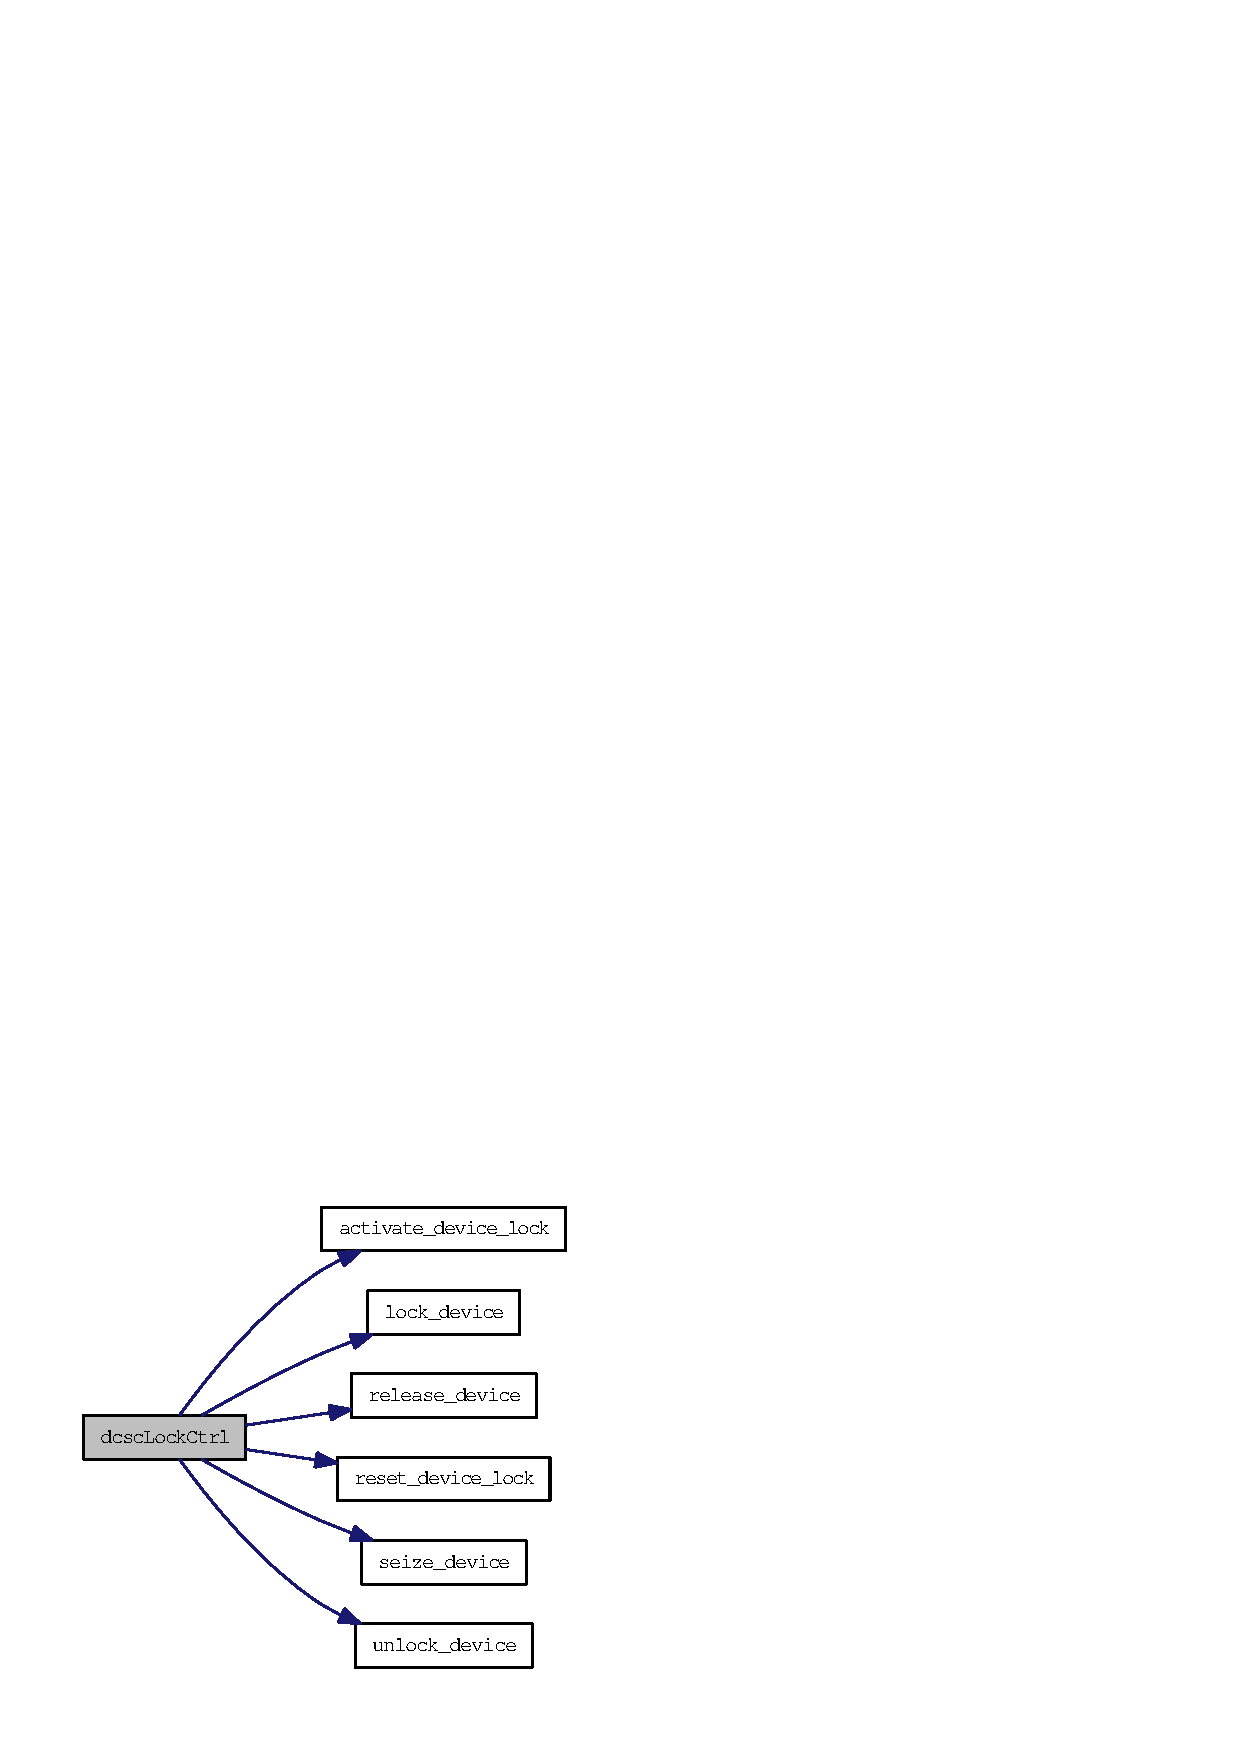
\includegraphics[width=138pt]{group__dcsc__msg__buffer__access_gb01774a452cb68f631a87d2d77ac79a5_cgraph}
\end{center}
\end{figure}
\hypertarget{group__dcsc__msg__buffer__access_g4f25fcb80c8fad99d5d72f96e72bd941}{
\index{dcsc_msg_buffer_access@{dcsc\_\-msg\_\-buffer\_\-access}!dcscPrepareMessageBuffer@{dcscPrepareMessageBuffer}}
\index{dcscPrepareMessageBuffer@{dcscPrepareMessageBuffer}!dcsc_msg_buffer_access@{dcsc\_\-msg\_\-buffer\_\-access}}
\subsubsection[dcscPrepareMessageBuffer]{\setlength{\rightskip}{0pt plus 5cm}int dcsc\-Prepare\-Message\-Buffer (\_\-\_\-u32 $\ast$$\ast$ {\em pp\-Buffer}, int $\ast$ {\em p\-Size}, unsigned int {\em cmd\-ID}, unsigned int {\em flags})}}
\label{group__dcsc__msg__buffer__access_g4f25fcb80c8fad99d5d72f96e72bd941}


Prepare the message buffer for a specific command. 

Creation and destruction of the buffer is handled by the interface internally {\bf DO NOT DELETE THIS BUFFER}.\par
 {\bf Note:} This function is forseen but not yet implemented \begin{Desc}
\item[Parameters:]
\begin{description}
\item[{\em pp\-Buffer}]target to receive the buffer pointer \item[{\em p\-Size}]target to receive the buffer size \item[{\em cmd\-ID}]command ID to prepare the buffer for \item[{\em flags}]for future extensions (e.g. preparation for compressed pedestal data) \end{description}
\end{Desc}
\begin{Desc}
\item[Returns:]pointer to buffer where the data words can directly be stored to, the information word and the markers and check sum are written by the interface. \end{Desc}


Definition at line 1600 of file dcsc\-Msg\-Buffer\-Interface.c.\hypertarget{group__dcsc__msg__buffer__access_gf7be7371f7530e8eb6e07e6f0d969b04}{
\index{dcsc_msg_buffer_access@{dcsc\_\-msg\_\-buffer\_\-access}!dcscProvideMessageBuffer@{dcscProvideMessageBuffer}}
\index{dcscProvideMessageBuffer@{dcscProvideMessageBuffer}!dcsc_msg_buffer_access@{dcsc\_\-msg\_\-buffer\_\-access}}
\subsubsection[dcscProvideMessageBuffer]{\setlength{\rightskip}{0pt plus 5cm}int dcsc\-Provide\-Message\-Buffer (\_\-\_\-u32 $\ast$$\ast$ {\em pp\-Buffer}, int $\ast$ {\em p\-Size})}}
\label{group__dcsc__msg__buffer__access_gf7be7371f7530e8eb6e07e6f0d969b04}


Provide the message buffer for direct access. 

Creation and destruction of the buffer is handled by the interface internally {\bf DO NOT DELETE THIS BUFFER}.\par
 {\bf Note:} This function is forseen but not yet implemented \begin{Desc}
\item[Parameters:]
\begin{description}
\item[{\em pp\-Buffer}]target to receive the buffer pointer \item[{\em p\-Size}]target to receive the buffer size \end{description}
\end{Desc}
\begin{Desc}
\item[Returns:]pointer to buffer, the caller is supposed to encode the complete message buffer, including the information word, the markers and data as well as check sum. The interface does not alter it. \end{Desc}


Definition at line 1575 of file dcsc\-Msg\-Buffer\-Interface.c.\hypertarget{group__dcsc__msg__buffer__access_gfc4448a8f5f9654cf54ad494f1558594}{
\index{dcsc_msg_buffer_access@{dcsc\_\-msg\_\-buffer\_\-access}!initRcuAccess@{initRcuAccess}}
\index{initRcuAccess@{initRcuAccess}!dcsc_msg_buffer_access@{dcsc\_\-msg\_\-buffer\_\-access}}
\subsubsection[initRcuAccess]{\setlength{\rightskip}{0pt plus 5cm}int init\-Rcu\-Access (const char $\ast$ {\em p\-Device\-Name})}}
\label{group__dcsc__msg__buffer__access_gfc4448a8f5f9654cf54ad494f1558594}


Initialize the interface. 

The device will be opened and some other other internal states initialized. \begin{Desc}
\item[Parameters:]
\begin{description}
\item[{\em p\-Device\-Name,:}]name of the device node, if NULL: /dev/dcsc as default \end{description}
\end{Desc}
\begin{Desc}
\item[Returns:]neg. error code if failed\par
 -ENOSPC : can not get the size of the interface buffers, or buffers too small\par
 -ENOENT : can not open device \end{Desc}


Definition at line 558 of file dcsc\-Msg\-Buffer\-Interface.c.

References init\-Rcu\-Access\-Ext().

Referenced by main().

Here is the call graph for this function:\begin{figure}[H]
\begin{center}
\leavevmode
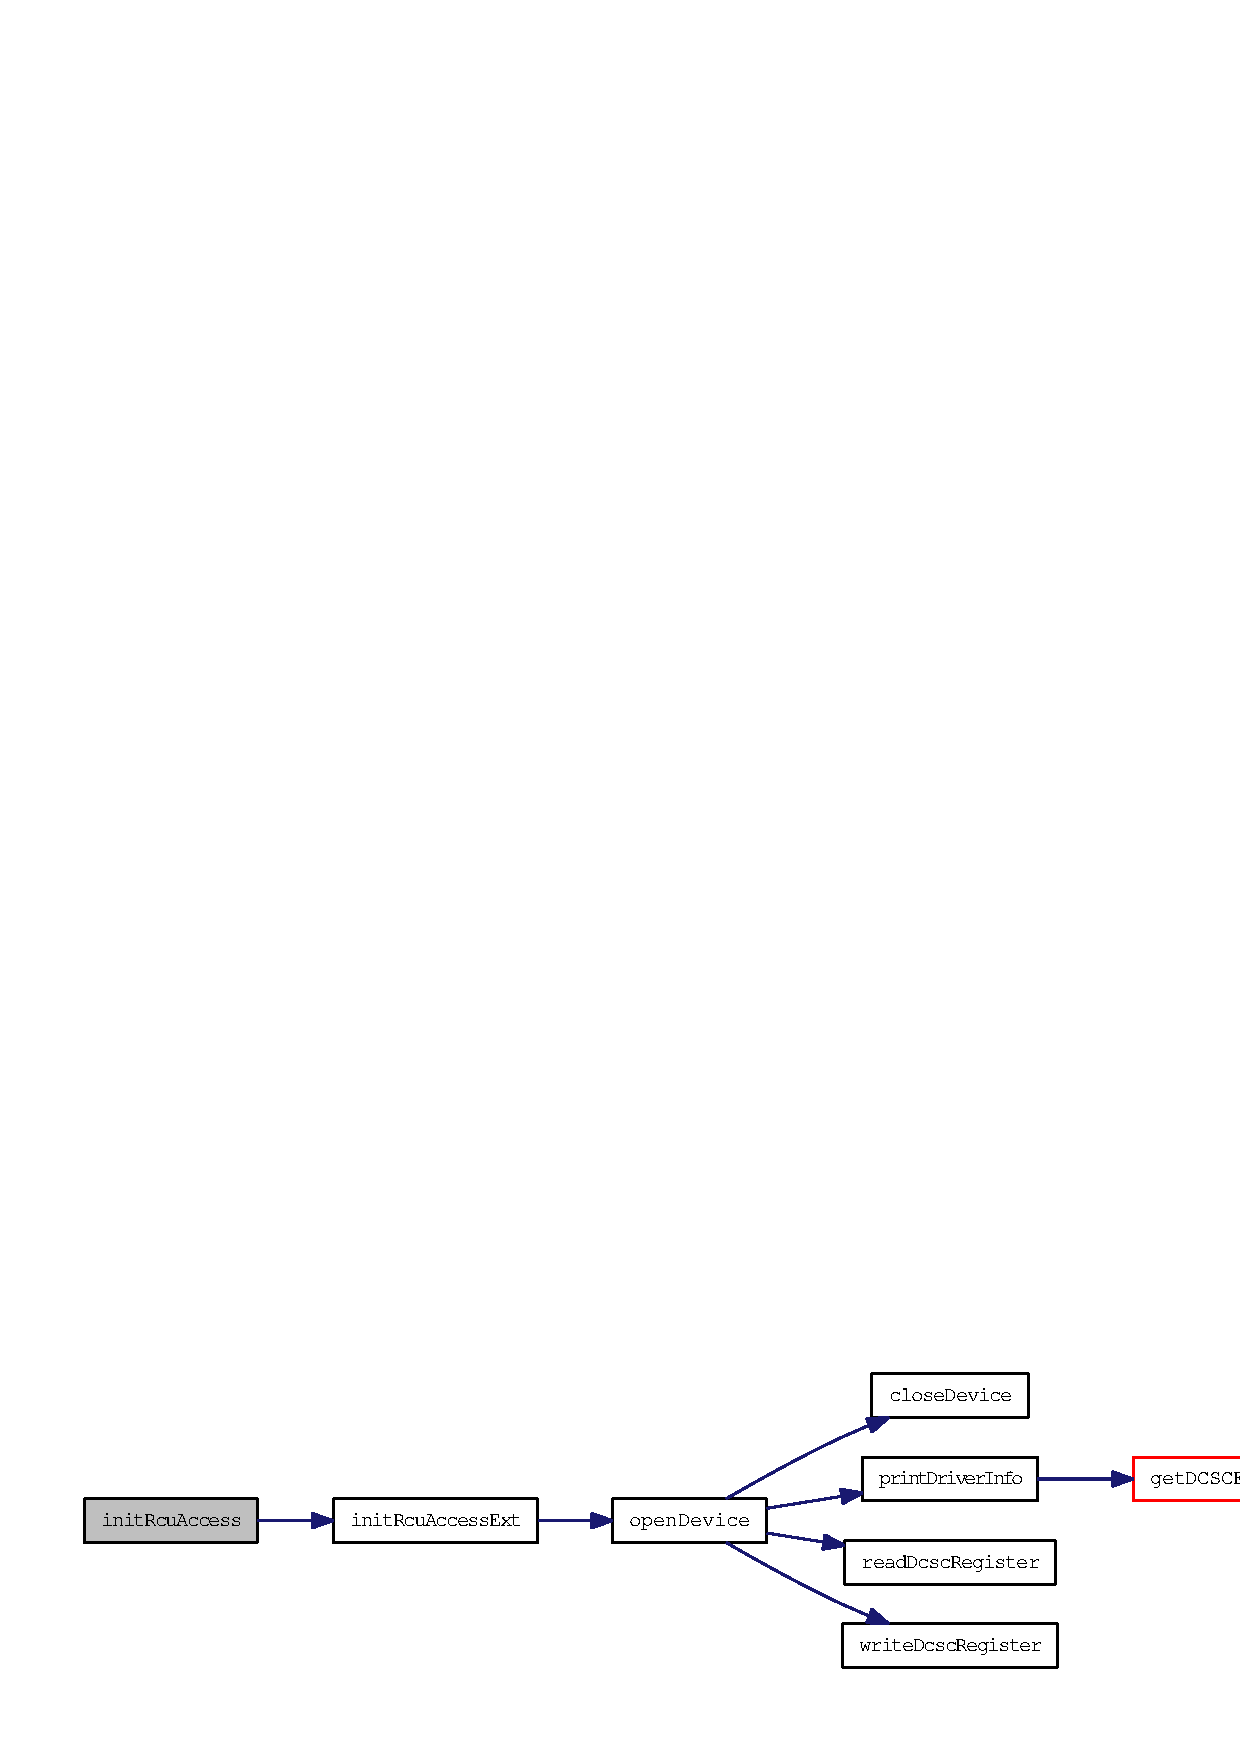
\includegraphics[width=350pt]{group__dcsc__msg__buffer__access_gfc4448a8f5f9654cf54ad494f1558594_cgraph}
\end{center}
\end{figure}
\hypertarget{group__dcsc__msg__buffer__access_g95f13464dd4da9231a53e7adbb0e7d4e}{
\index{dcsc_msg_buffer_access@{dcsc\_\-msg\_\-buffer\_\-access}!initRcuAccessExt@{initRcuAccessExt}}
\index{initRcuAccessExt@{initRcuAccessExt}!dcsc_msg_buffer_access@{dcsc\_\-msg\_\-buffer\_\-access}}
\subsubsection[initRcuAccessExt]{\setlength{\rightskip}{0pt plus 5cm}int init\-Rcu\-Access\-Ext (const char $\ast$ {\em p\-Device\-Name}, \hyperlink{structdcscInitArguments__t}{Tdcsc\-Init\-Arguments} $\ast$ {\em p\-Arg})}}
\label{group__dcsc__msg__buffer__access_g95f13464dd4da9231a53e7adbb0e7d4e}


Extended initialization. 

The function allows beside the device name a couple of other parameters to adjust the interface behavior. \begin{Desc}
\item[Parameters:]
\begin{description}
\item[{\em p\-Device\-Name}]name of the device node, if NULL: /dev/dcsc as default \item[{\em flags}]logical or of the following flags \item[{\em i\-MIBSize}]size of the MIB, used for encoding of message blocks \end{description}
\end{Desc}
\begin{Desc}
\item[Returns:]neg. error code if failed\par
 -ENOSPC : can not get the size of the interface buffers, or buffers too small\par
 -ENOENT : can not open device \end{Desc}


Definition at line 565 of file dcsc\-Msg\-Buffer\-Interface.c.

References DCSC\_\-INIT\_\-APPEND, DCSC\_\-INIT\_\-ENCODE, DCSC\_\-SKIP\_\-DRV\_\-ADPT, dcsc\-Init\-Arguments\_\-t::flags, g\_\-dcsc\-Flags, g\_\-verbosity, dcsc\-Init\-Arguments\_\-t::i\-MIBSize, dcsc\-Init\-Arguments\_\-t::i\-Verbosity, message\_\-in\_\-buffer\_\-size, and open\-Device().

Referenced by init\-Rcu\-Access(), and main().

Here is the call graph for this function:\begin{figure}[H]
\begin{center}
\leavevmode
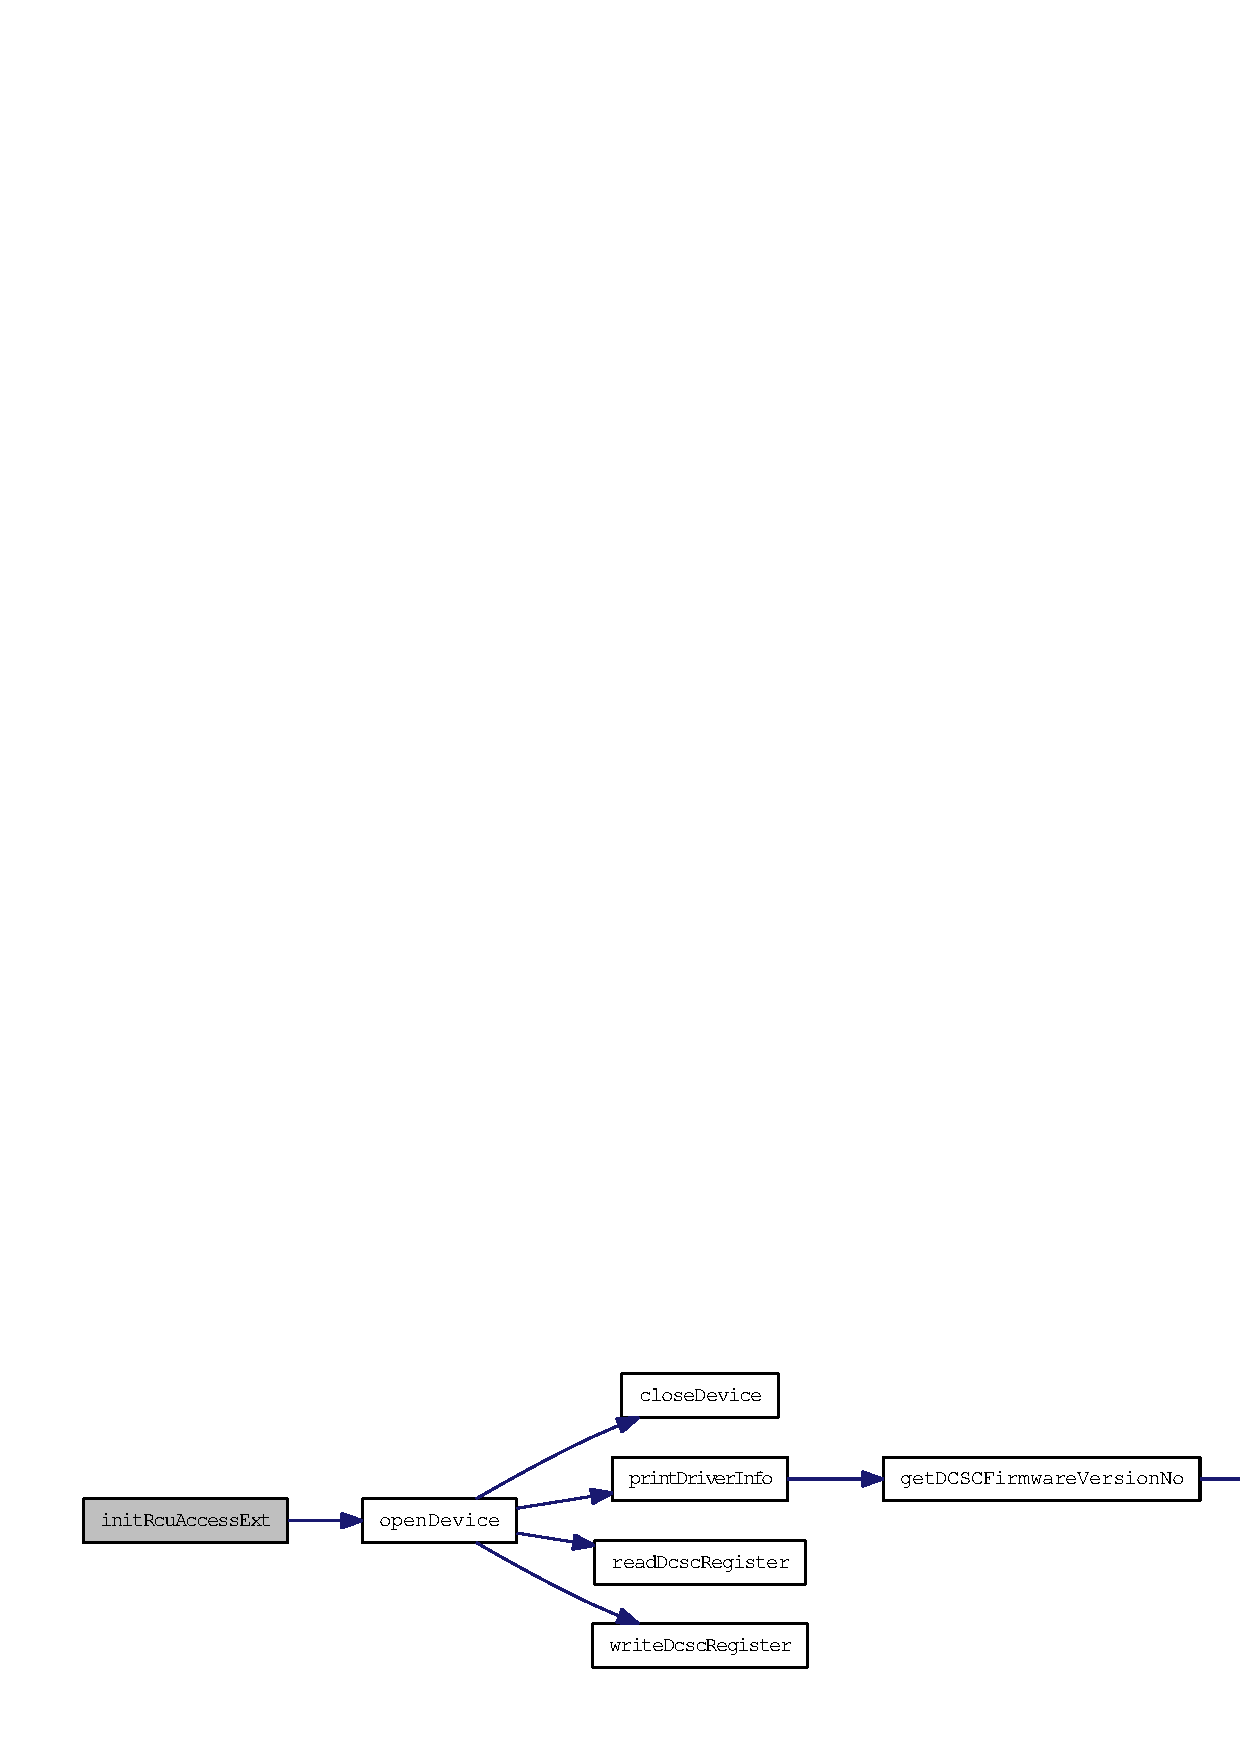
\includegraphics[width=351pt]{group__dcsc__msg__buffer__access_g95f13464dd4da9231a53e7adbb0e7d4e_cgraph}
\end{center}
\end{figure}
\hypertarget{group__dcsc__msg__buffer__access_g7a5b0d57fbd0a68206468a01b0a63520}{
\index{dcsc_msg_buffer_access@{dcsc\_\-msg\_\-buffer\_\-access}!msgBufReadRegister@{msgBufReadRegister}}
\index{msgBufReadRegister@{msgBufReadRegister}!dcsc_msg_buffer_access@{dcsc\_\-msg\_\-buffer\_\-access}}
\subsubsection[msgBufReadRegister]{\setlength{\rightskip}{0pt plus 5cm}int msg\-Buf\-Read\-Register (int {\em reg})}}
\label{group__dcsc__msg__buffer__access_g7a5b0d57fbd0a68206468a01b0a63520}


Read the value of a register from the register buffer. 

Originally, registers were 8 bit wide, but in the implementation of the message buffer interface in the DCS board firmware the addressing was 32 bit wide. Thats why register numbers correspond to register addresses = 4$\ast$reg\-No. \begin{Desc}
\item[Parameters:]
\begin{description}
\item[{\em reg}]\# of register \end{description}
\end{Desc}
\begin{Desc}
\item[Returns:]8 bit value of the register \end{Desc}


Definition at line 2078 of file dcsc\-Msg\-Buffer\-Interface.c.

References GENERAL\_\-CTRL\_\-REG\_\-ADDR, and read\-Dcsc\-Register().

Referenced by exec\-Reg\-Read\-Cmd().

Here is the call graph for this function:\begin{figure}[H]
\begin{center}
\leavevmode
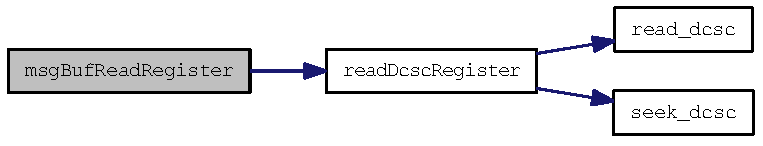
\includegraphics[width=201pt]{group__dcsc__msg__buffer__access_g7a5b0d57fbd0a68206468a01b0a63520_cgraph}
\end{center}
\end{figure}
\hypertarget{group__dcsc__msg__buffer__access_g82e19c9d34c7ecebcba115d2a6393b6c}{
\index{dcsc_msg_buffer_access@{dcsc\_\-msg\_\-buffer\_\-access}!msgBufWriteRegister@{msgBufWriteRegister}}
\index{msgBufWriteRegister@{msgBufWriteRegister}!dcsc_msg_buffer_access@{dcsc\_\-msg\_\-buffer\_\-access}}
\subsubsection[msgBufWriteRegister]{\setlength{\rightskip}{0pt plus 5cm}int msg\-Buf\-Write\-Register (int {\em reg}, unsigned char {\em value})}}
\label{group__dcsc__msg__buffer__access_g82e19c9d34c7ecebcba115d2a6393b6c}


Write an 8 bit value to a register of the register buffer. 

The same as in \hyperlink{group__dcsc__msg__buffer__access_g7a5b0d57fbd0a68206468a01b0a63520}{msg\-Buf\-Read\-Register} applies for the register addressing. \begin{Desc}
\item[Parameters:]
\begin{description}
\item[{\em reg}]\# of register \item[{\em value}]8 bit value to write \end{description}
\end{Desc}
\begin{Desc}
\item[Returns:]8 bit value of the register after write \end{Desc}


Definition at line 2086 of file dcsc\-Msg\-Buffer\-Interface.c.

References GENERAL\_\-CTRL\_\-REG\_\-ADDR, and write\-Dcsc\-Register().

Referenced by exec\-Reg\-Write\-Cmd().

Here is the call graph for this function:\begin{figure}[H]
\begin{center}
\leavevmode
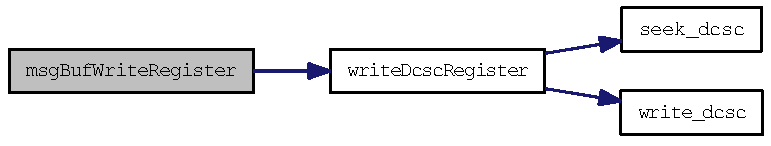
\includegraphics[width=203pt]{group__dcsc__msg__buffer__access_g82e19c9d34c7ecebcba115d2a6393b6c_cgraph}
\end{center}
\end{figure}
\hypertarget{group__dcsc__msg__buffer__access_g1b3027d209be85e9a8fbd14864c4b442}{
\index{dcsc_msg_buffer_access@{dcsc\_\-msg\_\-buffer\_\-access}!printBufferHex@{printBufferHex}}
\index{printBufferHex@{printBufferHex}!dcsc_msg_buffer_access@{dcsc\_\-msg\_\-buffer\_\-access}}
\subsubsection[printBufferHex]{\setlength{\rightskip}{0pt plus 5cm}void print\-Buffer\-Hex (unsigned char $\ast$ {\em p\-Buffer}, int {\em i\-Buffer\-Size}, int {\em word\-Size}, const char $\ast$ {\em p\-Message})}}
\label{group__dcsc__msg__buffer__access_g1b3027d209be85e9a8fbd14864c4b442}


Print content of a buffer hexadecimal. 

The content is assumed to be little endian (LSB first). \begin{Desc}
\item[Parameters:]
\begin{description}
\item[{\em p\-Buffer}]pointer to buffer \item[{\em i\-Buffer\-Size}]size of the buffer in byte \item[{\em i\-Word\-Size}]number of bytes in one word (1,2 or 4) \item[{\em p\-Message}]an optional message \end{description}
\end{Desc}


Definition at line 345 of file dcsc\-Msg\-Buffer\-Interface.c.

Referenced by check\-Msgin\-Buffer(), exec\-Write\-Cmd(), get\-Cmd\-Result(), print\-Buffer\-Hex\-Formatted(), rcu\-Flash\-ID(), rcu\-Multiple\-Read\-Ext(), rcu\-Single\-Read\-Ext(), and send\-Rcu\-Command().\hypertarget{group__dcsc__msg__buffer__access_gc44ca908f157f8de95b81638e298e08e}{
\index{dcsc_msg_buffer_access@{dcsc\_\-msg\_\-buffer\_\-access}!printBufferHexFormatted@{printBufferHexFormatted}}
\index{printBufferHexFormatted@{printBufferHexFormatted}!dcsc_msg_buffer_access@{dcsc\_\-msg\_\-buffer\_\-access}}
\subsubsection[printBufferHexFormatted]{\setlength{\rightskip}{0pt plus 5cm}void print\-Buffer\-Hex\-Formatted (unsigned char $\ast$ {\em p\-Buffer}, int {\em i\-Buffer\-Size}, int {\em i\-Word\-Size}, int {\em i\-Words\-Per\-Row}, int {\em i\-Start\-Address}, const char $\ast$ {\em p\-Message})}}
\label{group__dcsc__msg__buffer__access_gc44ca908f157f8de95b81638e298e08e}


Print content of a buffer hexadecimal formated with the address. 

The function formats the buffer to hexadecimal ascii with a dedicated number of words per row. Each row is preceeded by the address. The content is assumed to be little endian (LSB first) \begin{Desc}
\item[Parameters:]
\begin{description}
\item[{\em p\-Buffer}]pointer to buffer \item[{\em i\-Buffer\-Size}]size of the buffer in byte \item[{\em i\-Word\-Size}]number of bytes in one word (1,2 or 4) \item[{\em i\-Words\-Per\-Row}]number of words in one row \item[{\em i\-Start\-Address}]start address for the output \item[{\em p\-Message}]an optional message \end{description}
\end{Desc}


Definition at line 369 of file dcsc\-Msg\-Buffer\-Interface.c.

References print\-Buffer\-Hex().

Here is the call graph for this function:\begin{figure}[H]
\begin{center}
\leavevmode
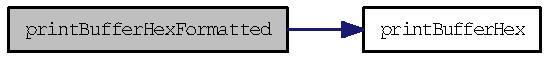
\includegraphics[width=150pt]{group__dcsc__msg__buffer__access_gc44ca908f157f8de95b81638e298e08e_cgraph}
\end{center}
\end{figure}
\hypertarget{group__dcsc__msg__buffer__access_g919bc832f5a0e82c07cfafd699b1b2ea}{
\index{dcsc_msg_buffer_access@{dcsc\_\-msg\_\-buffer\_\-access}!printDriverInfo@{printDriverInfo}}
\index{printDriverInfo@{printDriverInfo}!dcsc_msg_buffer_access@{dcsc\_\-msg\_\-buffer\_\-access}}
\subsubsection[printDriverInfo]{\setlength{\rightskip}{0pt plus 5cm}void print\-Driver\-Info (int {\em i\-Verbosity})}}
\label{group__dcsc__msg__buffer__access_g919bc832f5a0e82c07cfafd699b1b2ea}


Get driver info from the driver and print it. 

\begin{Desc}
\item[Parameters:]
\begin{description}
\item[{\em i\-Verbosity}]1 full text, 0 just a few messages \end{description}
\end{Desc}


Definition at line 1839 of file dcsc\-Msg\-Buffer\-Interface.c.

References DCSC\_\-REQUIRED\_\-DRIVER\_\-VERSION\_\-MAJOR, DCSC\_\-REQUIRED\_\-DRIVER\_\-VERSION\_\-MINOR, g\_\-file, get\-DCSCFirmware\-Version\-No(), IOCTL\_\-GET\_\-VERS\_\-STR\_\-SIZE, IOCTL\_\-GET\_\-VERSION, IOCTL\_\-GET\_\-VERSION\_\-V02, message\_\-in\_\-buffer\_\-size, message\_\-out\_\-buffer\_\-size, message\_\-regfile\_\-size, RCUBUS\_\-DRIVER\_\-VERSION\_\-MAJOR\_\-BITSHIFT, RCUBUS\_\-DRIVER\_\-VERSION\_\-MAJOR\_\-SIZE, RCUBUS\_\-DRIVER\_\-VERSION\_\-MINOR\_\-BITSHIFT, and RCUBUS\_\-DRIVER\_\-VERSION\_\-MINOR\_\-SIZE.

Referenced by open\-Device().

Here is the call graph for this function:\begin{figure}[H]
\begin{center}
\leavevmode
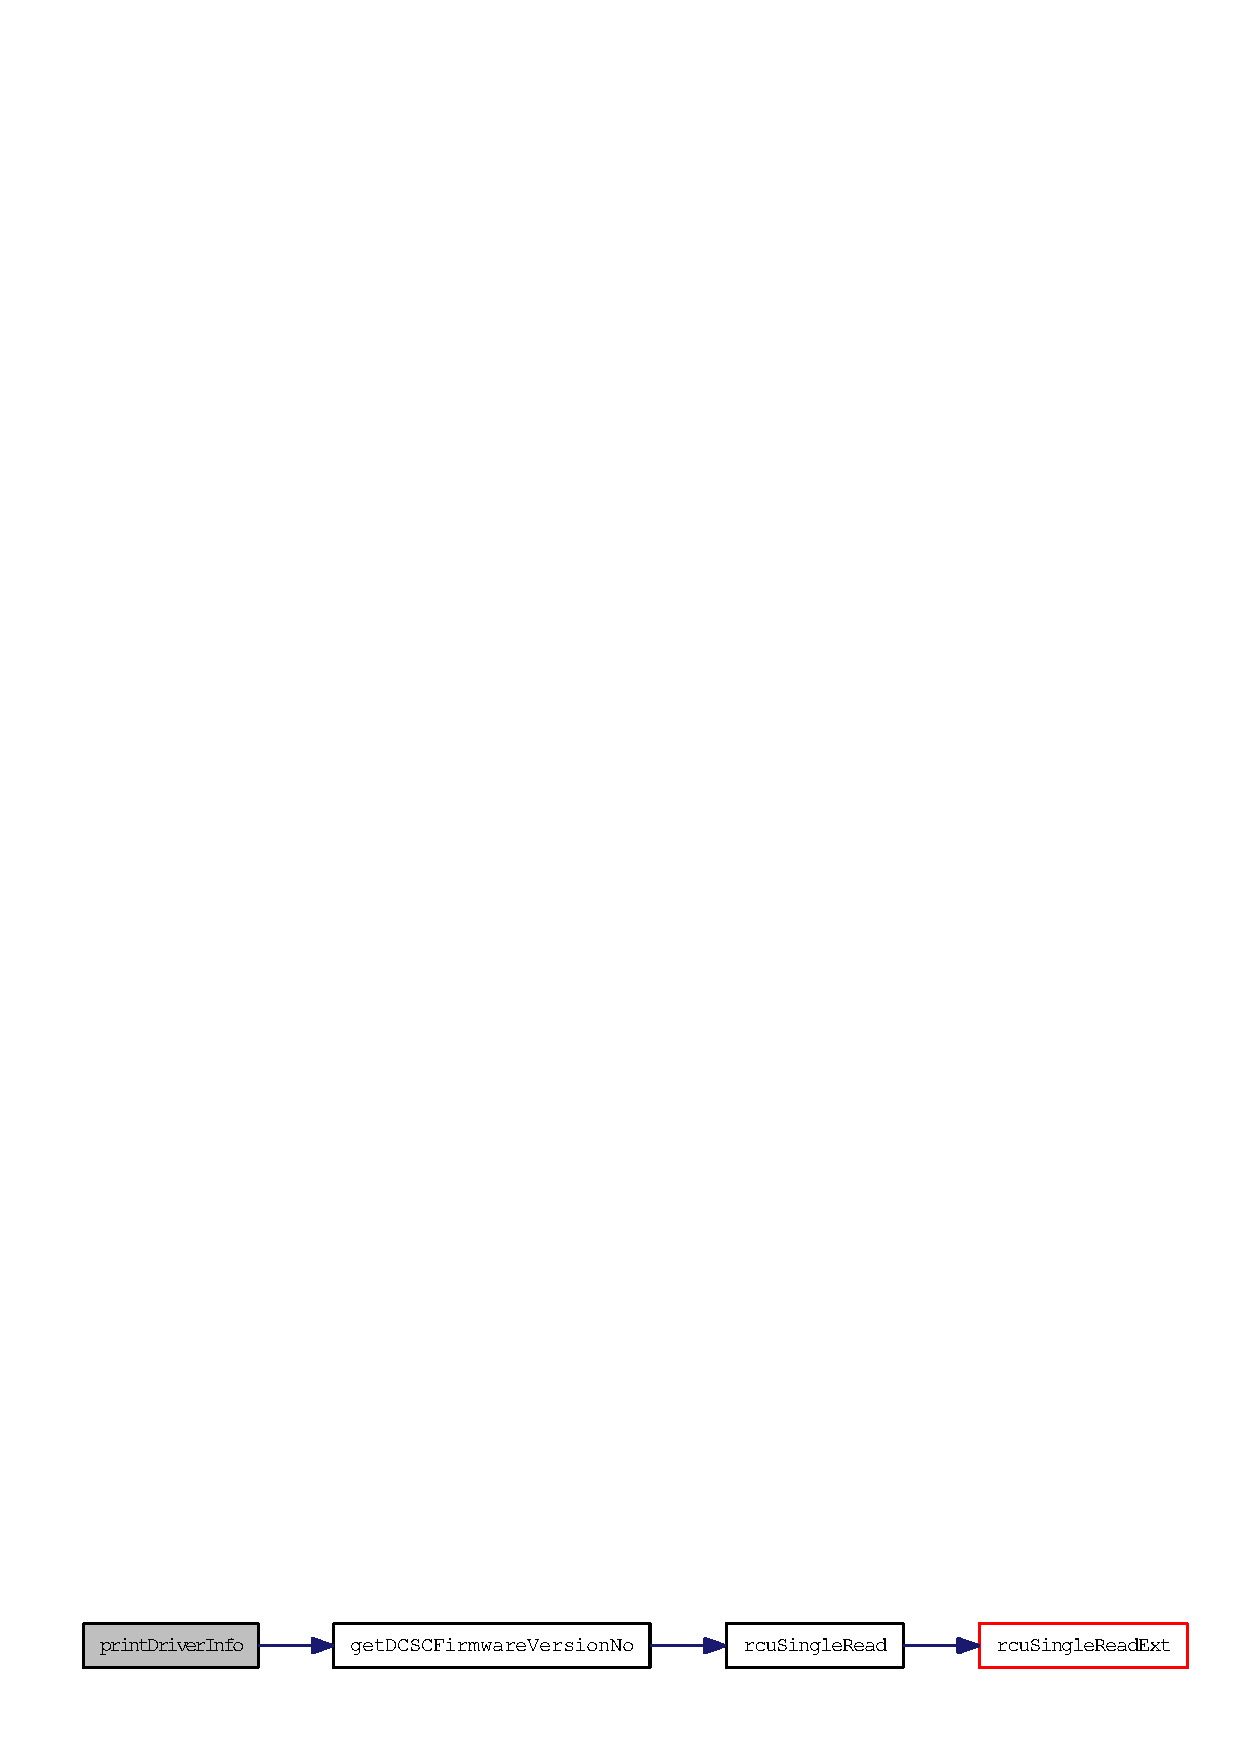
\includegraphics[width=287pt]{group__dcsc__msg__buffer__access_g919bc832f5a0e82c07cfafd699b1b2ea_cgraph}
\end{center}
\end{figure}
\hypertarget{group__dcsc__msg__buffer__access_gf74b29f8ded2feb57974c95e4863eac8}{
\index{dcsc_msg_buffer_access@{dcsc\_\-msg\_\-buffer\_\-access}!rcuBusControlCmd@{rcuBusControlCmd}}
\index{rcuBusControlCmd@{rcuBusControlCmd}!dcsc_msg_buffer_access@{dcsc\_\-msg\_\-buffer\_\-access}}
\subsubsection[rcuBusControlCmd]{\setlength{\rightskip}{0pt plus 5cm}int rcu\-Bus\-Control\-Cmd (int {\em i\-Cmd})}}
\label{group__dcsc__msg__buffer__access_gf74b29f8ded2feb57974c95e4863eac8}


Switch bits in the control register (firmware comstat). 

\begin{Desc}
\item[Parameters:]
\begin{description}
\item[{\em i\-Cmd}]buffer control command, see enums above \end{description}
\end{Desc}
\begin{Desc}
\item[Returns:]the (new) value of the control register, neg. error code if failed\par
 -EBADFD if interface in wrong state to perform the command\par
 -EIO if internal error (bits can not be changed)\par
 -EINVAL unknown command id \end{Desc}


Definition at line 2073 of file dcsc\-Msg\-Buffer\-Interface.c.

References rcu\-Bus\-Control\-Cmd\-Ext().

Referenced by calculate\-Stop\-Address(), ctrl\-Reg\-Status(), enter\-Flash\-State(), get\-Bus\-State(), and restore\-Bus\-State().

Here is the call graph for this function:\begin{figure}[H]
\begin{center}
\leavevmode
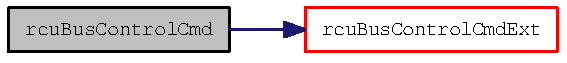
\includegraphics[width=154pt]{group__dcsc__msg__buffer__access_gf74b29f8ded2feb57974c95e4863eac8_cgraph}
\end{center}
\end{figure}
\hypertarget{group__dcsc__msg__buffer__access_g78e6fc883a098cf548e9d0ba618ecb16}{
\index{dcsc_msg_buffer_access@{dcsc\_\-msg\_\-buffer\_\-access}!rcuFlashErase@{rcuFlashErase}}
\index{rcuFlashErase@{rcuFlashErase}!dcsc_msg_buffer_access@{dcsc\_\-msg\_\-buffer\_\-access}}
\subsubsection[rcuFlashErase]{\setlength{\rightskip}{0pt plus 5cm}int rcu\-Flash\-Erase (int {\em start\-Sec}, int {\em stop\-Sec})}}
\label{group__dcsc__msg__buffer__access_g78e6fc883a098cf548e9d0ba618ecb16}


Erase sectors of the flash. 

\begin{Desc}
\item[Parameters:]
\begin{description}
\item[{\em first\-Sec}]the first sector to erase; if -1 erase all \item[{\em last\-Sec}]the last sector to erase \end{description}
\end{Desc}
\begin{Desc}
\item[Returns:]0 success, neg. error code if failed \end{Desc}


Definition at line 2311 of file dcsc\-Msg\-Buffer\-Interface.c.

References check\-State(), e\-Disable\-Flash, e\-Enable\-Flash, e\-Flash, e\-Flash\-Access\-Dcsc, FLASH\_\-ERASE\_\-SEC, FLASH\_\-ERASEALL, FLASH\_\-MULTI\_\-ERASE, g\_\-i\-Flash\-Access\-Mode, g\_\-verbosity, lock\_\-device(), mib\-Size, mk\-End\-Marker(), mk\-Frst\-Wrd(), mk\-Lst\-Wrd(), MSGBUF\_\-MODE\_\-FLASH, p\-Mib, RCU\_\-FLASH\_\-ADDRH, RCU\_\-FLASH\_\-ADDRL, RCU\_\-FLASH\_\-CMD, RCU\_\-FLASH\_\-ERASE\_\-WAITCYCLE, RCU\_\-FLASH\_\-ERASEALL, RCU\_\-FLASH\_\-ERASESEC, RCU\_\-FLASH\_\-MAX\_\-WAITSTATES, RCU\_\-FLASH\_\-STATE\_\-IDLE, RCU\_\-FLASH\_\-STATE\_\-MASK, RCU\_\-FLASH\_\-STATUS, rcu\-Bus\-Control\-Cmd\-Ext(), rcu\-Single\-Read(), rcu\-Single\-Write(), send\-Rcu\-Command(), and unlock\_\-device().

Referenced by exec\-Flash\-Erase(), exec\-Flash\-Eraseall(), and main().

Here is the call graph for this function:\begin{figure}[H]
\begin{center}
\leavevmode
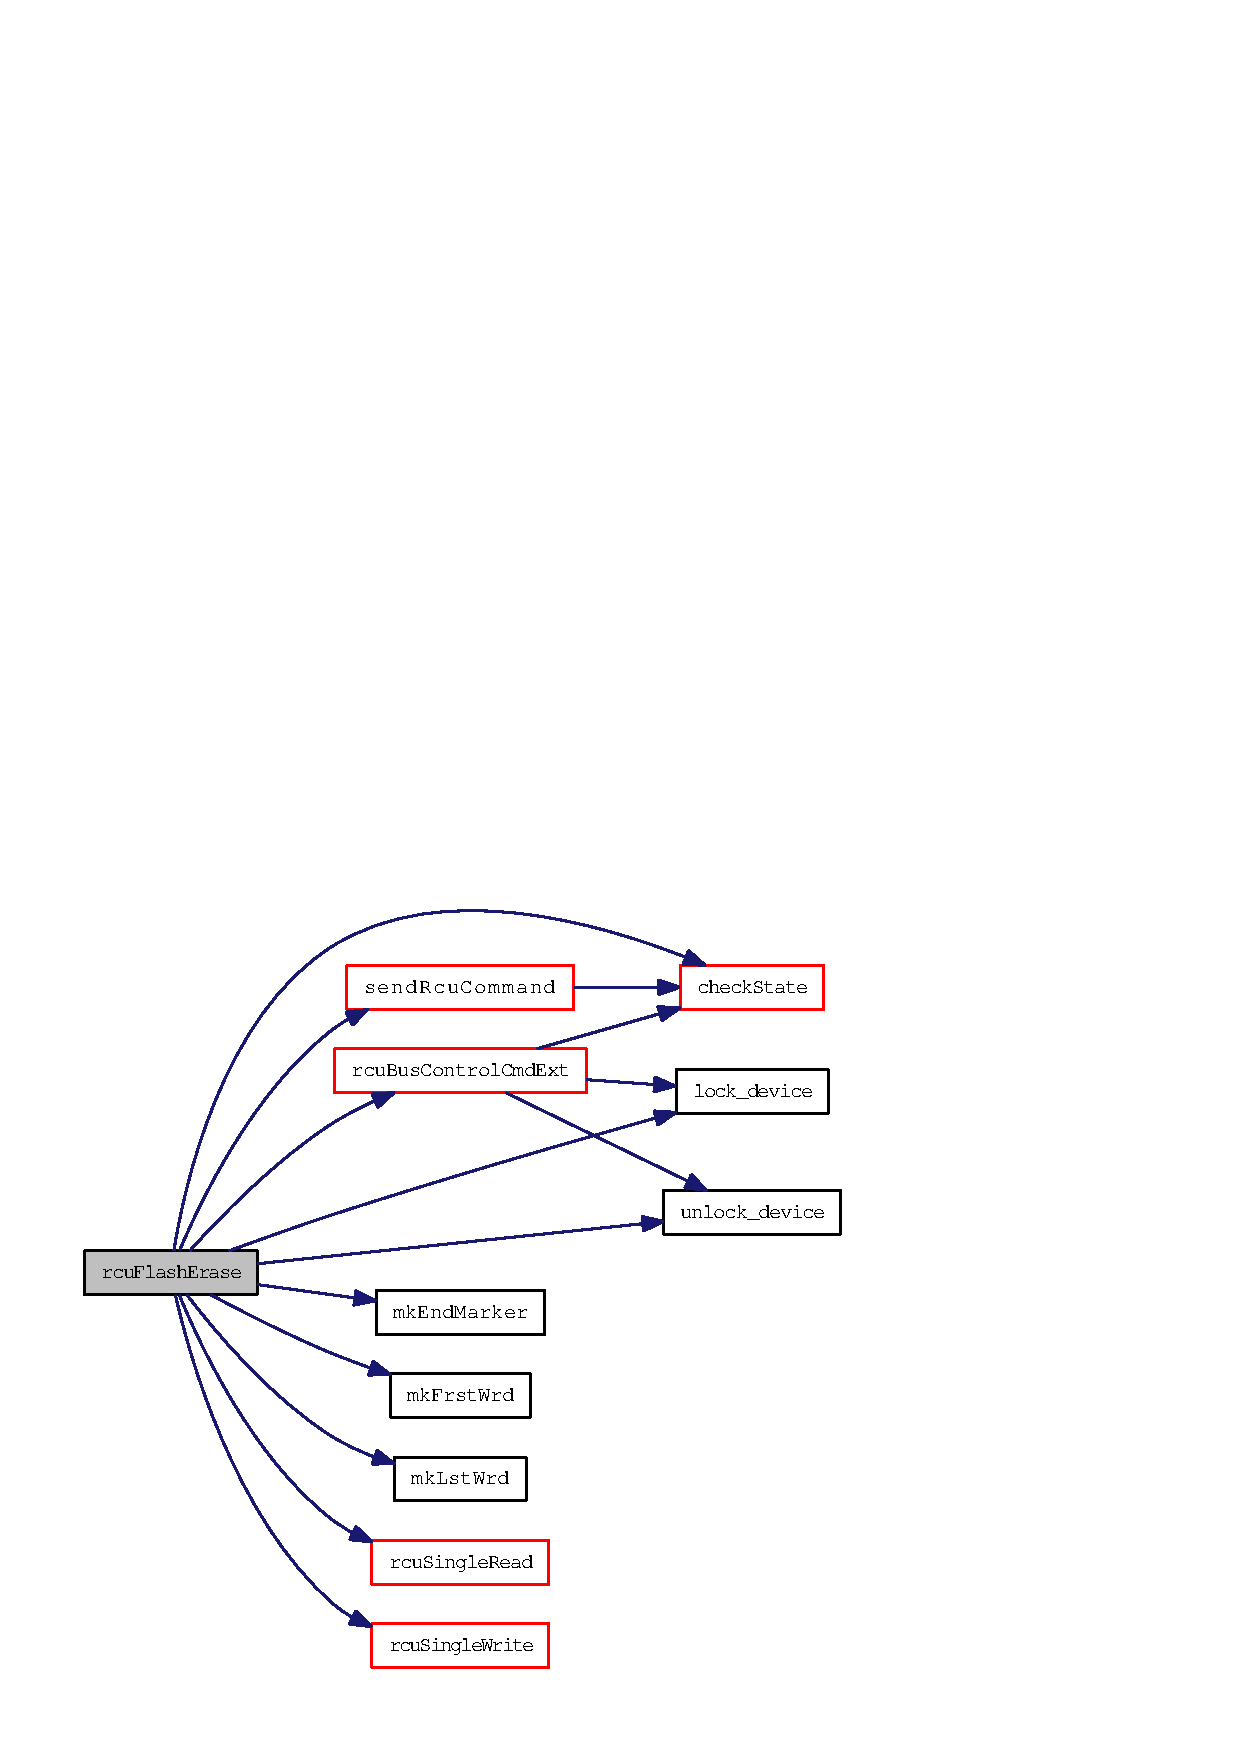
\includegraphics[width=204pt]{group__dcsc__msg__buffer__access_g78e6fc883a098cf548e9d0ba618ecb16_cgraph}
\end{center}
\end{figure}
\hypertarget{group__dcsc__msg__buffer__access_g24164f14711ead31a7e542711f0a08b3}{
\index{dcsc_msg_buffer_access@{dcsc\_\-msg\_\-buffer\_\-access}!rcuFlashRead@{rcuFlashRead}}
\index{rcuFlashRead@{rcuFlashRead}!dcsc_msg_buffer_access@{dcsc\_\-msg\_\-buffer\_\-access}}
\subsubsection[rcuFlashRead]{\setlength{\rightskip}{0pt plus 5cm}int rcu\-Flash\-Read (\_\-\_\-u32 {\em address}, int {\em i\-Size}, \_\-\_\-u32 $\ast$ {\em p\-Data})}}
\label{group__dcsc__msg__buffer__access_g24164f14711ead31a7e542711f0a08b3}


Read a number of 16bit words from the flash memory. 

currently all communication is done through the message buffer \begin{Desc}
\item[Parameters:]
\begin{description}
\item[{\em address}]start location \item[{\em i\-Size}]number of words to read \item[{\em p\-Data}]buffer to receive the data, the function expect it to be of suitable size (i.e. i\-Size x wordsize) \end{description}
\end{Desc}
\begin{Desc}
\item[Returns:]number of read 32bit words, neg. error code if failed \end{Desc}


Definition at line 2223 of file dcsc\-Msg\-Buffer\-Interface.c.

References check\-State(), e\-Disable\-Flash, e\-Enable\-Flash, e\-Flash, e\-Flash\-Access\-Dcsc, g\_\-i\-Flash\-Access\-Mode, g\_\-verbosity, lock\_\-device(), MSGBUF\_\-MODE\_\-FLASH, RCU\_\-FLASH\_\-ADDRH, RCU\_\-FLASH\_\-ADDRL, RCU\_\-FLASH\_\-AHBSHFT, RCU\_\-FLASH\_\-AHMASK, RCU\_\-FLASH\_\-ALMASK, RCU\_\-FLASH\_\-CMD, RCU\_\-FLASH\_\-DEFAULT\_\-WAITCYCLE, RCU\_\-FLASH\_\-MAX\_\-WAITSTATES, RCU\_\-FLASH\_\-READCMD, RCU\_\-FLASH\_\-READRES, RCU\_\-FLASH\_\-SIZE, RCU\_\-FLASH\_\-STATE\_\-IDLE, RCU\_\-FLASH\_\-STATE\_\-MASK, RCU\_\-FLASH\_\-STATUS, rcu\-Bus\-Control\-Cmd\-Ext(), rcu\-Multiple\-Read\-Ext(), rcu\-Single\-Read(), rcu\-Single\-Write(), and unlock\_\-device().

Referenced by exec\-Read\-Cmd(), and exec\-Write\-Cmd().

Here is the call graph for this function:\begin{figure}[H]
\begin{center}
\leavevmode
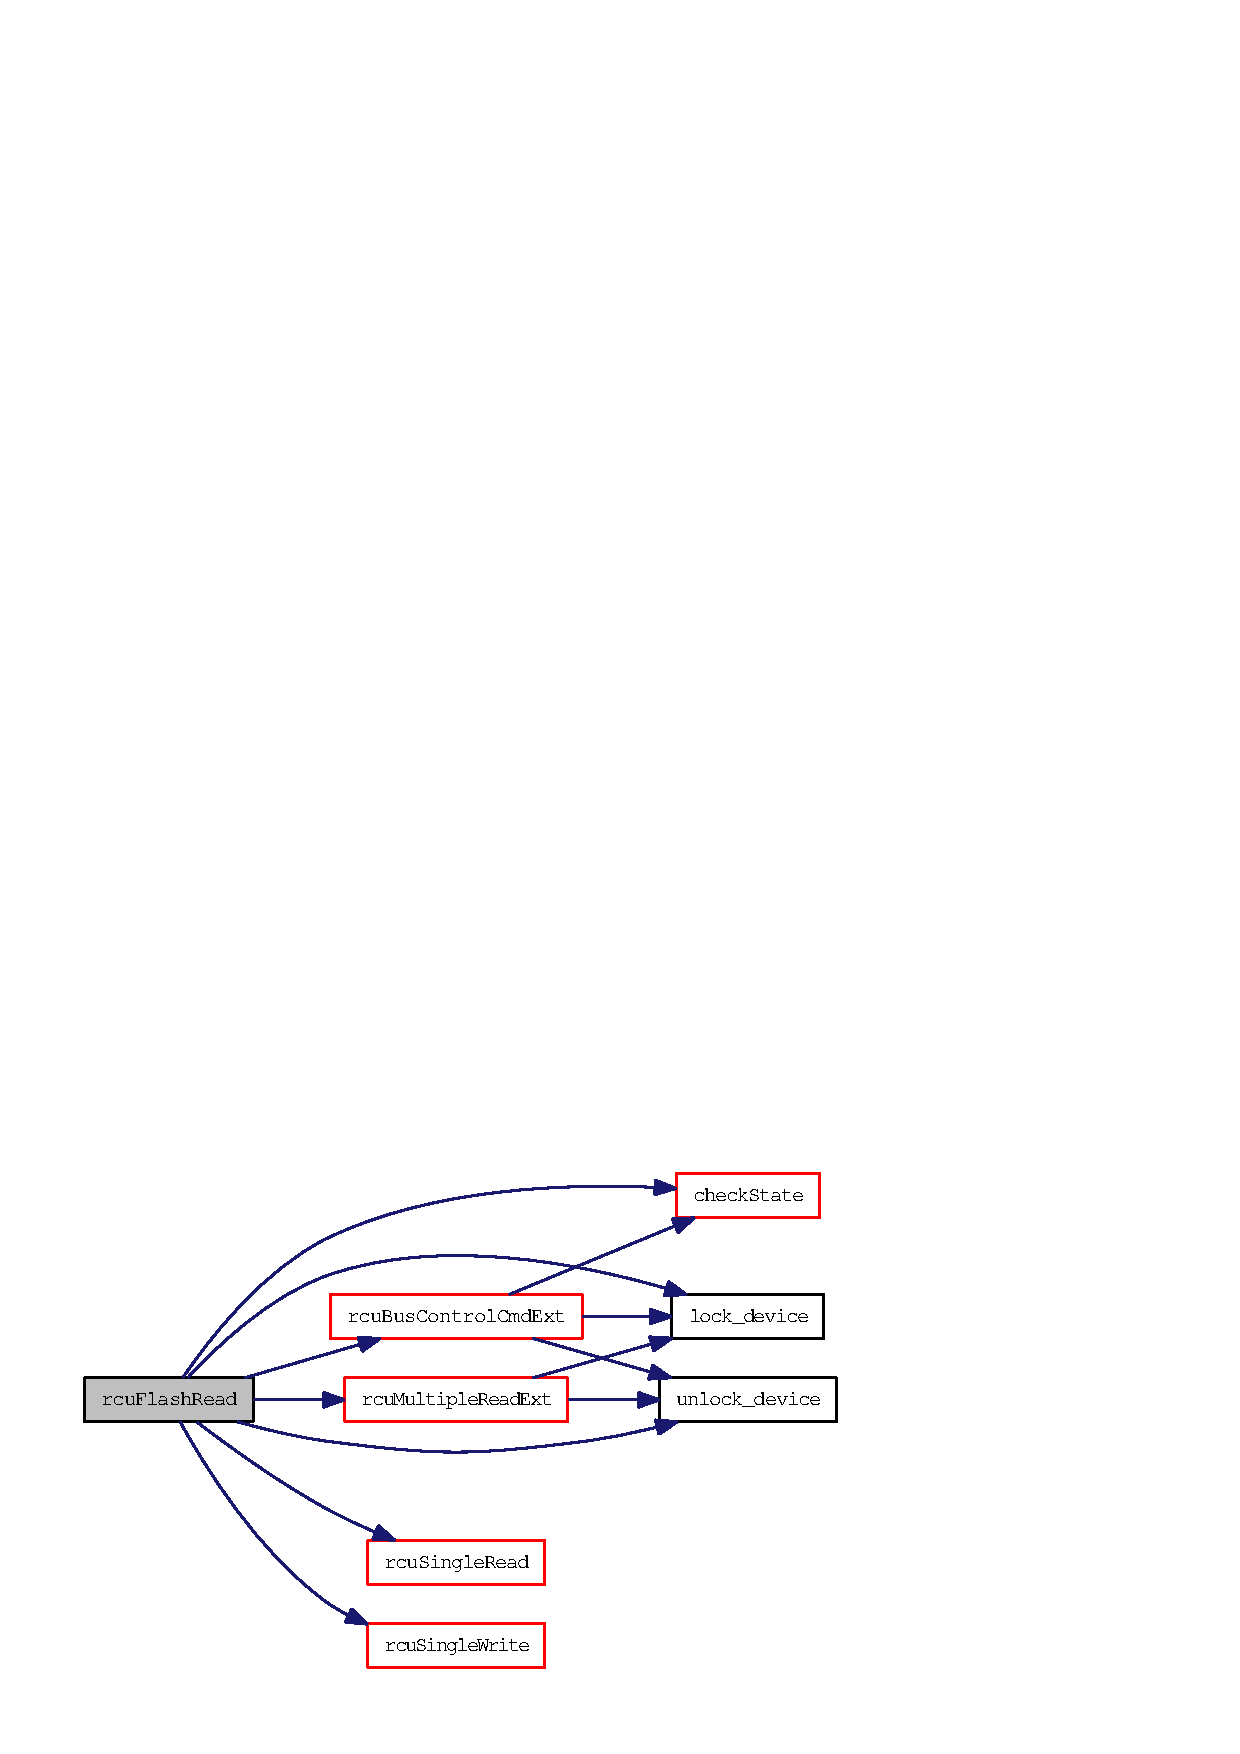
\includegraphics[width=203pt]{group__dcsc__msg__buffer__access_g24164f14711ead31a7e542711f0a08b3_cgraph}
\end{center}
\end{figure}
\hypertarget{group__dcsc__msg__buffer__access_g88debbd24075d2031add9459e4d90e2b}{
\index{dcsc_msg_buffer_access@{dcsc\_\-msg\_\-buffer\_\-access}!rcuFlashWrite@{rcuFlashWrite}}
\index{rcuFlashWrite@{rcuFlashWrite}!dcsc_msg_buffer_access@{dcsc\_\-msg\_\-buffer\_\-access}}
\subsubsection[rcuFlashWrite]{\setlength{\rightskip}{0pt plus 5cm}int rcu\-Flash\-Write (\_\-\_\-u32 {\em address}, \_\-\_\-u32 $\ast$ {\em p\-Data}, int {\em i\-Size}, int {\em i\-Data\-Size})}}
\label{group__dcsc__msg__buffer__access_g88debbd24075d2031add9459e4d90e2b}


Write to the RCU flash. 

currently all communication is done through the message buffer \begin{Desc}
\item[Parameters:]
\begin{description}
\item[{\em address}]start location \item[{\em p\-Data}]buffer containing the data \item[{\em i\-Size}]number of words to write \item[{\em i\-Data\-Size}]size of one word in bytes, allowed 1,2 \end{description}
\end{Desc}
\begin{Desc}
\item[Returns:]\end{Desc}


Definition at line 2130 of file dcsc\-Msg\-Buffer\-Interface.c.

References check\-State(), e\-Disable\-Flash, e\-Enable\-Flash, e\-Flash, e\-Flash\-Access\-Dcsc, g\_\-i\-Flash\-Access\-Mode, g\_\-verbosity, lock\_\-device(), MSGBUF\_\-MODE\_\-FLASH, RCU\_\-FLASH\_\-ADDRH, RCU\_\-FLASH\_\-ADDRL, RCU\_\-FLASH\_\-AHBSHFT, RCU\_\-FLASH\_\-AHMASK, RCU\_\-FLASH\_\-ALMASK, RCU\_\-FLASH\_\-CMD, RCU\_\-FLASH\_\-DATA, RCU\_\-FLASH\_\-DEFAULT\_\-WAITCYCLE, RCU\_\-FLASH\_\-MAX\_\-WAITSTATES, RCU\_\-FLASH\_\-SIZE, RCU\_\-FLASH\_\-STATE\_\-IDLE, RCU\_\-FLASH\_\-STATE\_\-MASK, RCU\_\-FLASH\_\-STATUS, RCU\_\-FLASH\_\-WRITECMD, rcu\-Bus\-Control\-Cmd\-Ext(), rcu\-Multiple\-Write\-Ext(), rcu\-Single\-Read(), rcu\-Single\-Write(), and unlock\_\-device().

Referenced by do\-Flash\-Frame(), do\-Init(), do\-Scrubbing(), and exec\-Write\-Cmd().

Here is the call graph for this function:\begin{figure}[H]
\begin{center}
\leavevmode
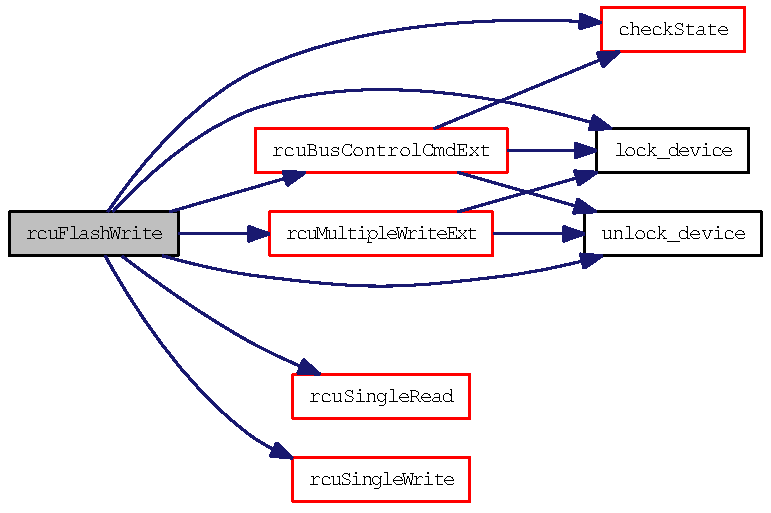
\includegraphics[width=203pt]{group__dcsc__msg__buffer__access_g88debbd24075d2031add9459e4d90e2b_cgraph}
\end{center}
\end{figure}
\hypertarget{group__dcsc__msg__buffer__access_g602216accce6913989f8b04b36157cd6}{
\index{dcsc_msg_buffer_access@{dcsc\_\-msg\_\-buffer\_\-access}!rcuMultipleRead@{rcuMultipleRead}}
\index{rcuMultipleRead@{rcuMultipleRead}!dcsc_msg_buffer_access@{dcsc\_\-msg\_\-buffer\_\-access}}
\subsubsection[rcuMultipleRead]{\setlength{\rightskip}{0pt plus 5cm}int rcu\-Multiple\-Read (\_\-\_\-u32 {\em address}, int {\em i\-Size}, \_\-\_\-u32 $\ast$ {\em p\-Data})}}
\label{group__dcsc__msg__buffer__access_g602216accce6913989f8b04b36157cd6}


Read a number of 32bit words beginning at a location. 

\begin{Desc}
\item[Parameters:]
\begin{description}
\item[{\em address}]16 bit address in RCU memory space \item[{\em i\-Size}]number of words to write \item[{\em p\-Data}]buffer to receive the data, the function expect it to be of suitable size (i.e. i\-Size x wordsize) \end{description}
\end{Desc}
\begin{Desc}
\item[Returns:]number of 32bit words which have been read, neg. error code if failed \end{Desc}


Definition at line 1566 of file dcsc\-Msg\-Buffer\-Interface.c.

References MSGBUF\_\-MODE\_\-MEMMAPPED, and rcu\-Multiple\-Read\-Ext().

Referenced by exec\-Read\-Cmd(), and main().

Here is the call graph for this function:\begin{figure}[H]
\begin{center}
\leavevmode
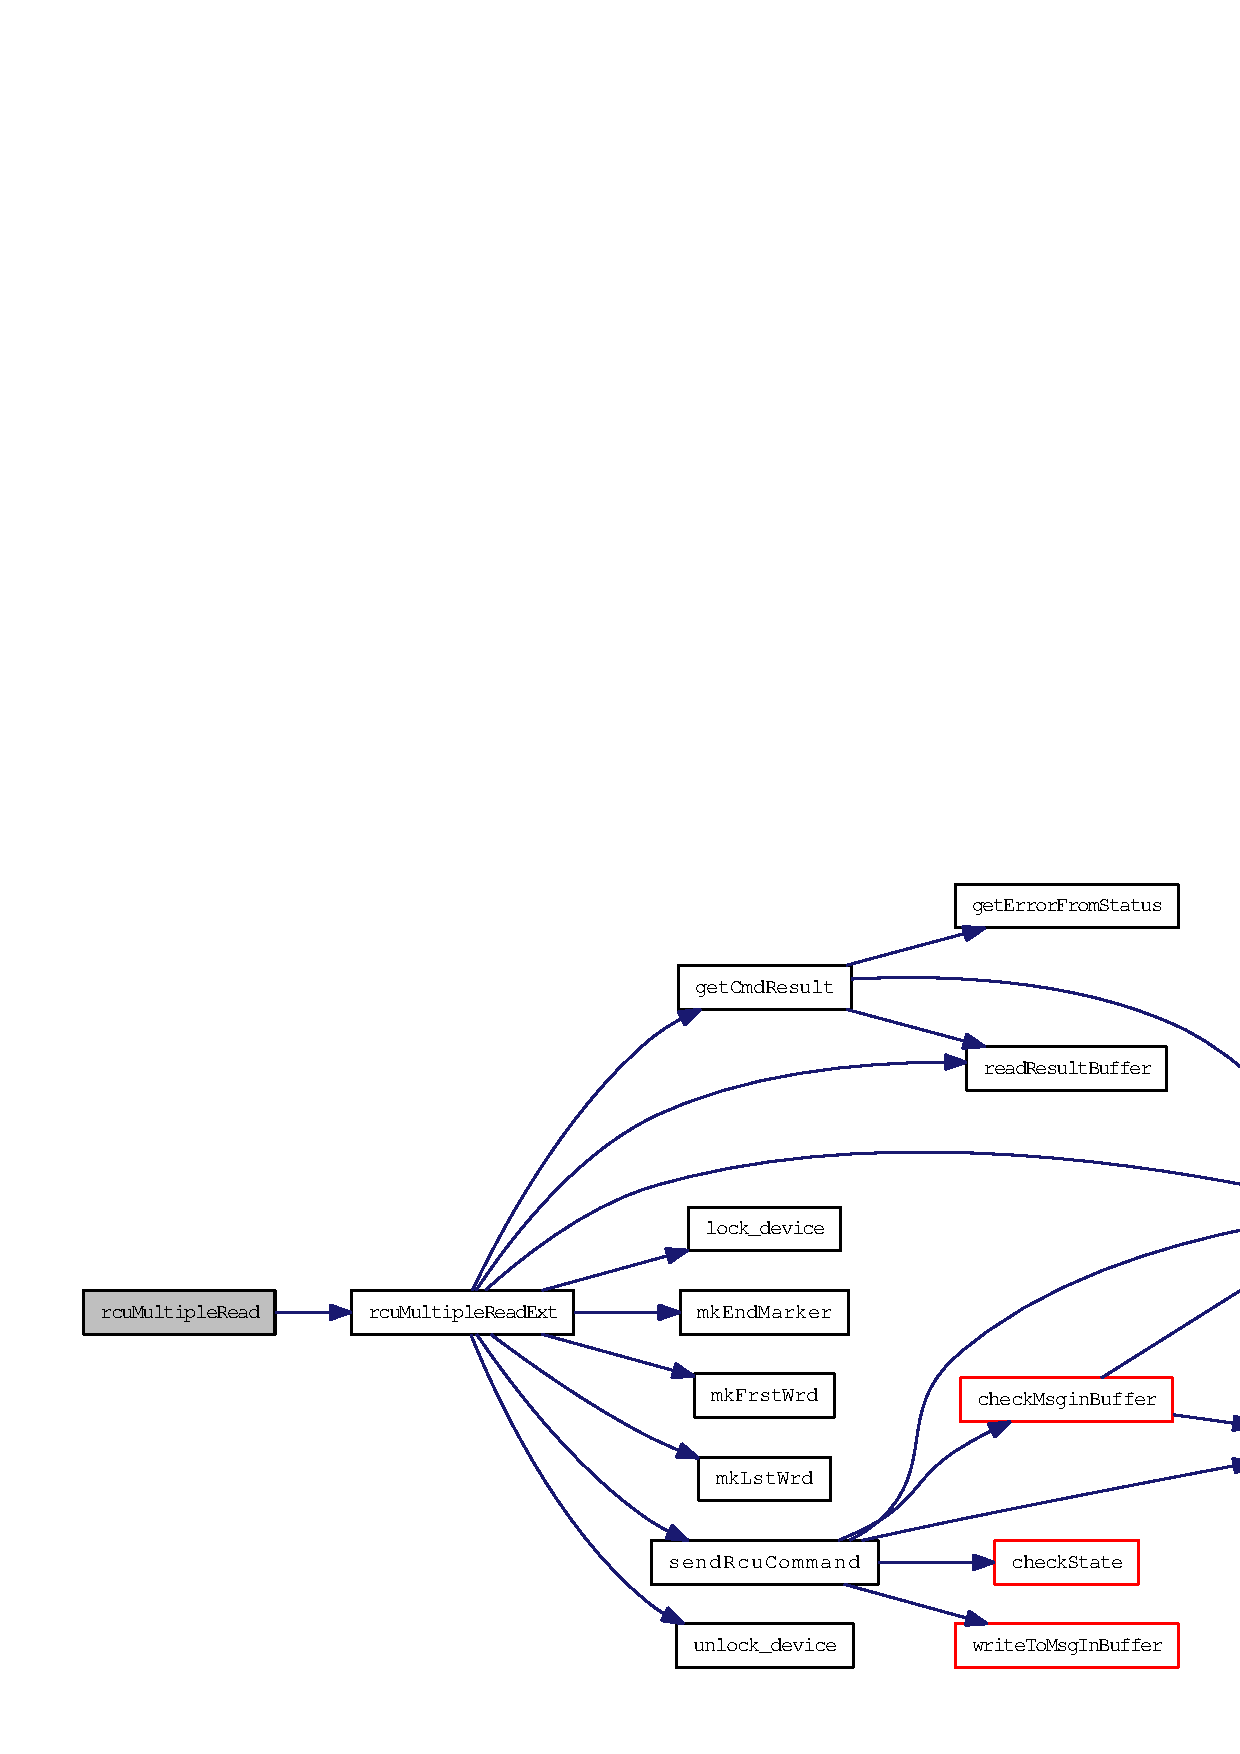
\includegraphics[width=356pt]{group__dcsc__msg__buffer__access_g602216accce6913989f8b04b36157cd6_cgraph}
\end{center}
\end{figure}
\hypertarget{group__dcsc__msg__buffer__access_ge20afbfc92c897546e37126188804309}{
\index{dcsc_msg_buffer_access@{dcsc\_\-msg\_\-buffer\_\-access}!rcuMultipleWrite@{rcuMultipleWrite}}
\index{rcuMultipleWrite@{rcuMultipleWrite}!dcsc_msg_buffer_access@{dcsc\_\-msg\_\-buffer\_\-access}}
\subsubsection[rcuMultipleWrite]{\setlength{\rightskip}{0pt plus 5cm}int rcu\-Multiple\-Write (\_\-\_\-u32 {\em address}, \_\-\_\-u32 $\ast$ {\em p\-Data}, int {\em i\-Size}, int {\em i\-Data\-Size})}}
\label{group__dcsc__msg__buffer__access_ge20afbfc92c897546e37126188804309}


Write a number of 32bit words beginning at a location. 

The function takes care for the size of the MIB and splits the operation if the amount of data to write exceeds the MIB size. The function expects data in little endian byte order \begin{Desc}
\item[Parameters:]
\begin{description}
\item[{\em address}]16 bit address in RCU memory space \item[{\em p\-Data}]buffer containing the data \item[{\em i\-Size}]number of words to write \item[{\em i\-Data\-Size}]size of one word in bytes, allowed 1 (8 bit), 2 (16 bit),3 (compressed 10 bit) or 4 (32 bit) -2 and -4 denote 16/32 bit words which get swapped \end{description}
\end{Desc}
\begin{Desc}
\item[Returns:]\end{Desc}


Definition at line 1549 of file dcsc\-Msg\-Buffer\-Interface.c.

References MSGBUF\_\-MODE\_\-MEMMAPPED, and rcu\-Multiple\-Write\-Ext().

Referenced by exec\-Write\-Cmd(), and init().

Here is the call graph for this function:\begin{figure}[H]
\begin{center}
\leavevmode
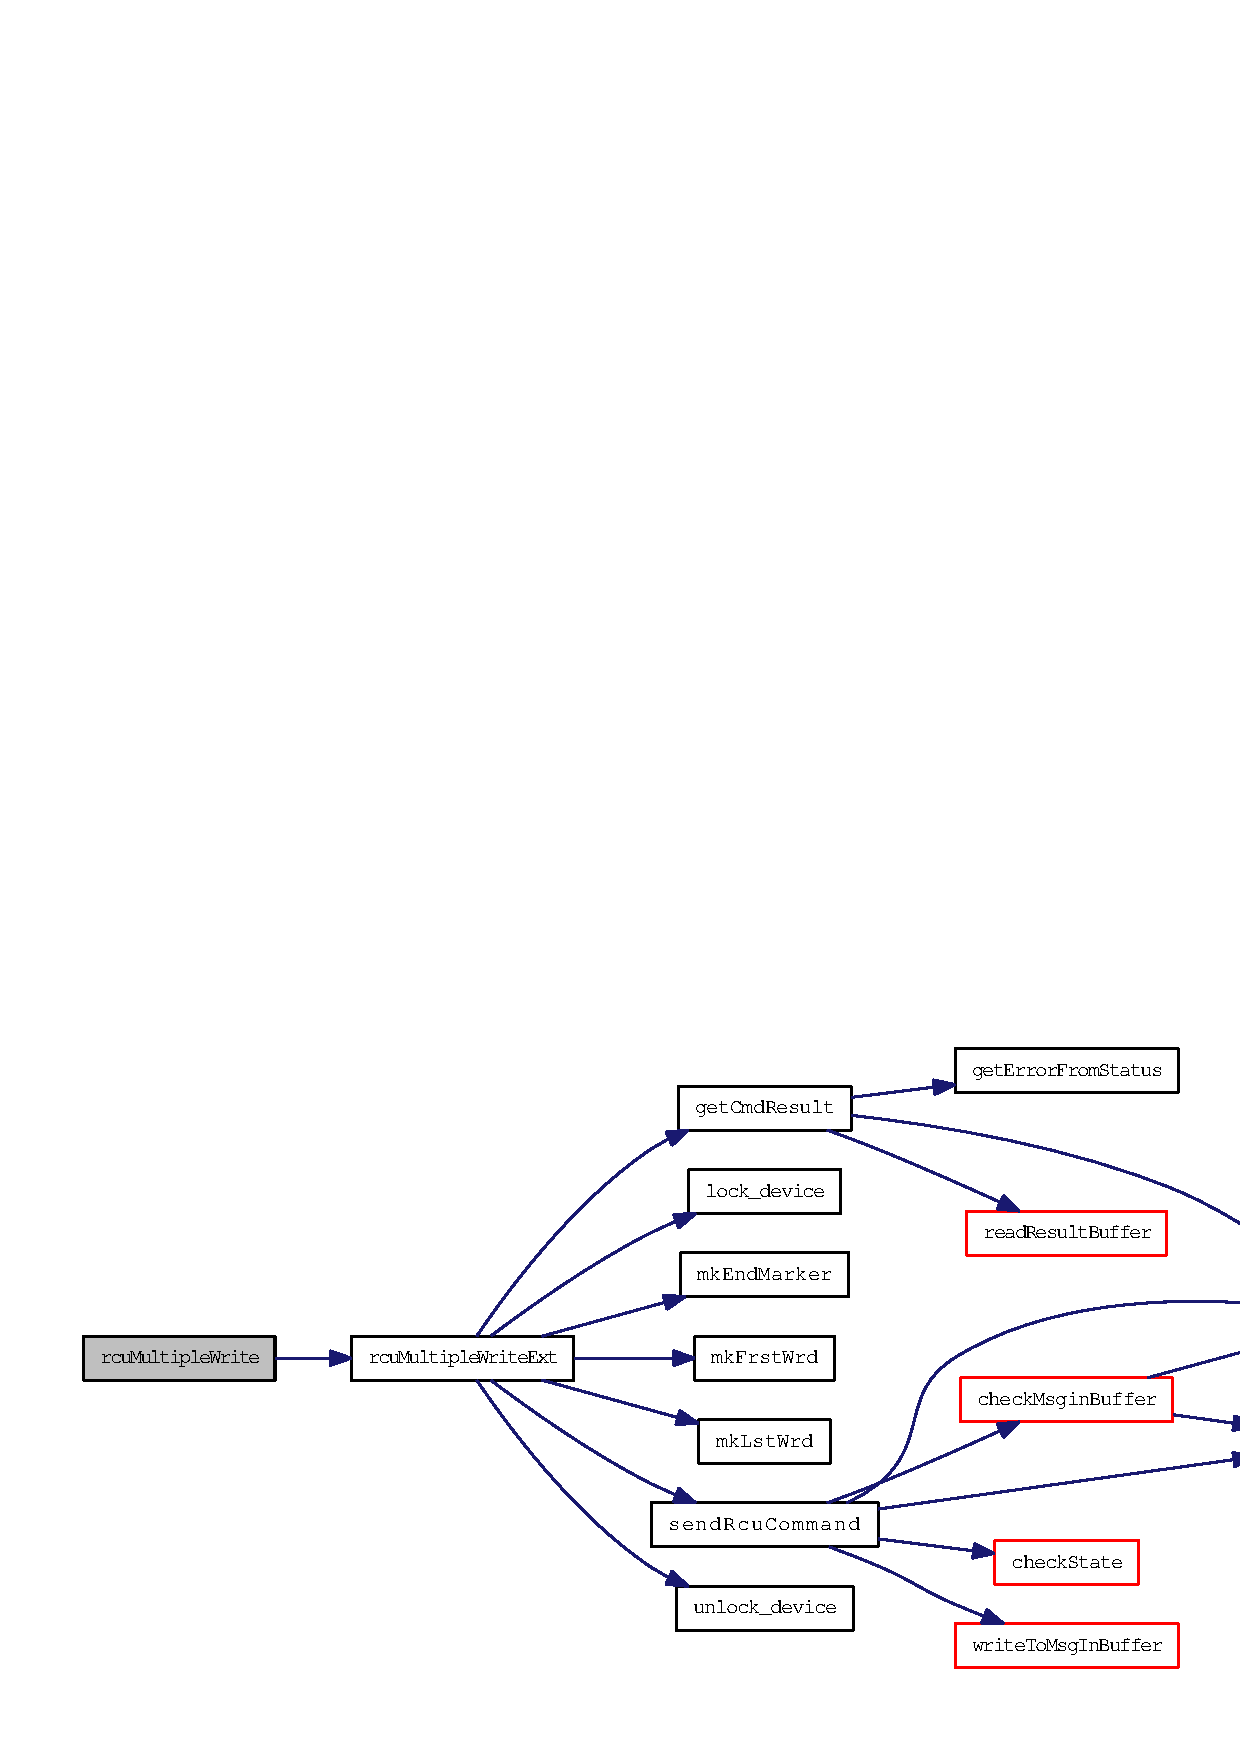
\includegraphics[width=356pt]{group__dcsc__msg__buffer__access_ge20afbfc92c897546e37126188804309_cgraph}
\end{center}
\end{figure}
\hypertarget{group__dcsc__msg__buffer__access_g339b5922513d0f0211d7962234faa24f}{
\index{dcsc_msg_buffer_access@{dcsc\_\-msg\_\-buffer\_\-access}!rcuSingleRead@{rcuSingleRead}}
\index{rcuSingleRead@{rcuSingleRead}!dcsc_msg_buffer_access@{dcsc\_\-msg\_\-buffer\_\-access}}
\subsubsection[rcuSingleRead]{\setlength{\rightskip}{0pt plus 5cm}int rcu\-Single\-Read (\_\-\_\-u32 {\em address}, \_\-\_\-u32 $\ast$ {\em p\-Data})}}
\label{group__dcsc__msg__buffer__access_g339b5922513d0f0211d7962234faa24f}


Read a single location (32bit word). 

\begin{Desc}
\item[Parameters:]
\begin{description}
\item[{\em address}]16 bit address in RCU memory space \item[{\em p\-Data}]buffer to receive the data \end{description}
\end{Desc}
\begin{Desc}
\item[Returns:]\end{Desc}


Definition at line 1557 of file dcsc\-Msg\-Buffer\-Interface.c.

References MSGBUF\_\-MODE\_\-MEMMAPPED, and rcu\-Single\-Read\-Ext().

Referenced by calculate\-Stop\-Address(), exec\-Read\-Cmd(), get\-DCSCFirmware\-Version\-No(), get\-Errorcounter\-Reg(), get\-Last\-Error\-Framenumber(), get\-Last\-Framenumber(), get\-Number\-Of\-Cycles(), rcu\-Flash\-Erase(), rcu\-Flash\-ID(), rcu\-Flash\-Read(), rcu\-Flash\-Reset(), rcu\-Flash\-Write(), read\-Err\-Reg(), read\-Status\-Reg(), and wait\-Condition().

Here is the call graph for this function:\begin{figure}[H]
\begin{center}
\leavevmode
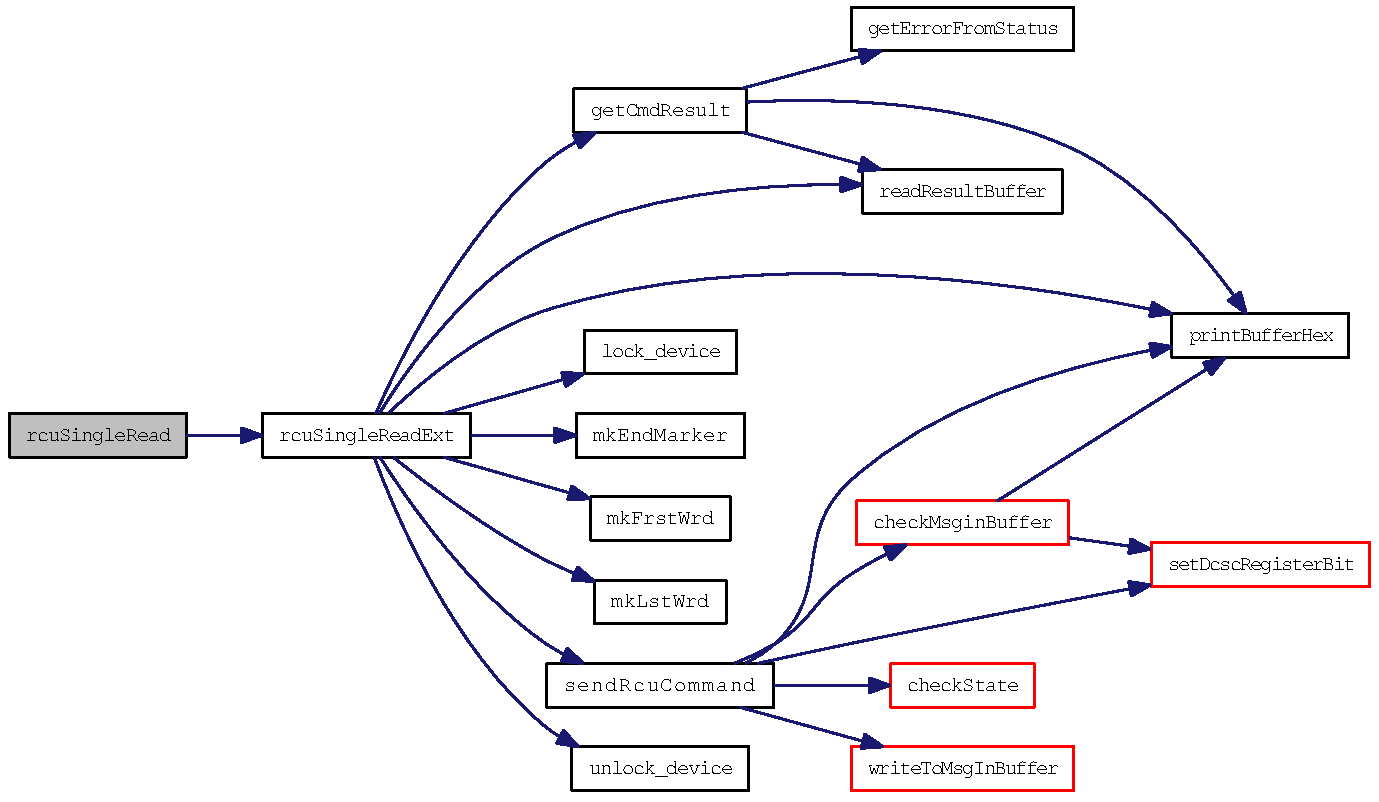
\includegraphics[width=349pt]{group__dcsc__msg__buffer__access_g339b5922513d0f0211d7962234faa24f_cgraph}
\end{center}
\end{figure}
\hypertarget{group__dcsc__msg__buffer__access_g5b2ecab6b0a6383afebde1ea486dae43}{
\index{dcsc_msg_buffer_access@{dcsc\_\-msg\_\-buffer\_\-access}!rcuSingleWrite@{rcuSingleWrite}}
\index{rcuSingleWrite@{rcuSingleWrite}!dcsc_msg_buffer_access@{dcsc\_\-msg\_\-buffer\_\-access}}
\subsubsection[rcuSingleWrite]{\setlength{\rightskip}{0pt plus 5cm}int rcu\-Single\-Write (\_\-\_\-u32 {\em address}, \_\-\_\-u32 {\em data})}}
\label{group__dcsc__msg__buffer__access_g5b2ecab6b0a6383afebde1ea486dae43}


Write a single location (32bit word). 

\begin{Desc}
\item[Parameters:]
\begin{description}
\item[{\em address}]16 bit address in RCU memory space \item[{\em data}]data word \end{description}
\end{Desc}
\begin{Desc}
\item[Returns:]\end{Desc}


Definition at line 1541 of file dcsc\-Msg\-Buffer\-Interface.c.

References MSGBUF\_\-MODE\_\-MEMMAPPED, and rcu\-Single\-Write\-Ext().

Referenced by clear\-Err\-Reg(), commit(), exec\-Write\-Cmd(), init(), main(), rcu\-Flash\-Erase(), rcu\-Flash\-ID(), rcu\-Flash\-Read(), rcu\-Flash\-Reset(), rcu\-Flash\-Write(), and step().

Here is the call graph for this function:\begin{figure}[H]
\begin{center}
\leavevmode
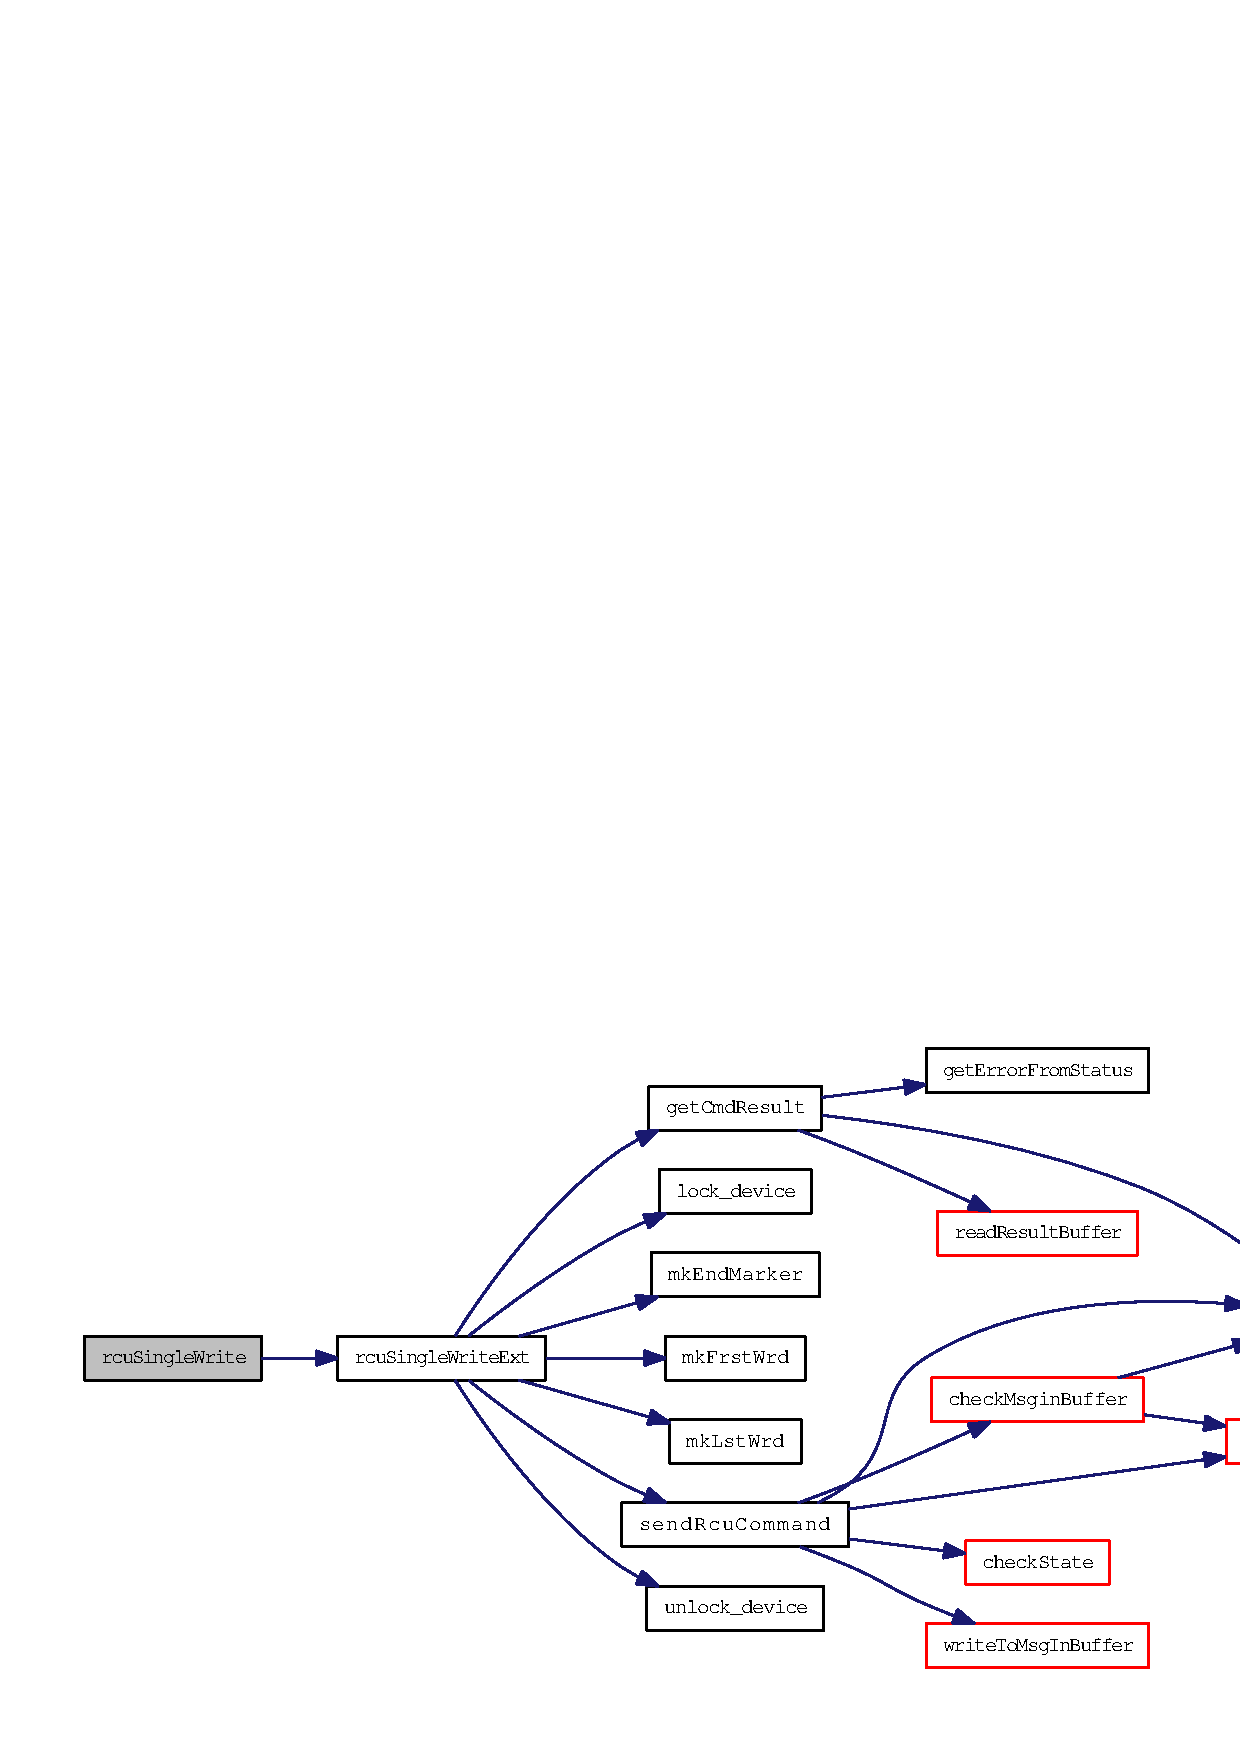
\includegraphics[width=349pt]{group__dcsc__msg__buffer__access_g5b2ecab6b0a6383afebde1ea486dae43_cgraph}
\end{center}
\end{figure}
\hypertarget{group__dcsc__msg__buffer__access_gac62a9e57c67af4cb9178b4426ec12fb}{
\index{dcsc_msg_buffer_access@{dcsc\_\-msg\_\-buffer\_\-access}!releaseRcuAccess@{releaseRcuAccess}}
\index{releaseRcuAccess@{releaseRcuAccess}!dcsc_msg_buffer_access@{dcsc\_\-msg\_\-buffer\_\-access}}
\subsubsection[releaseRcuAccess]{\setlength{\rightskip}{0pt plus 5cm}int release\-Rcu\-Access ()}}
\label{group__dcsc__msg__buffer__access_gac62a9e57c67af4cb9178b4426ec12fb}


Close the device and release internal data structures. 

\begin{Desc}
\item[Returns:]neg. error code if failed \par
 -ENXIO : no device open \end{Desc}


Definition at line 597 of file dcsc\-Msg\-Buffer\-Interface.c.

References close\-Device().

Referenced by main().

Here is the call graph for this function:\begin{figure}[H]
\begin{center}
\leavevmode
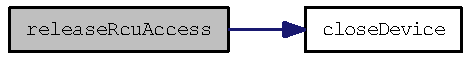
\includegraphics[width=131pt]{group__dcsc__msg__buffer__access_gac62a9e57c67af4cb9178b4426ec12fb_cgraph}
\end{center}
\end{figure}
\hypertarget{group__dcsc__msg__buffer__access_gb54d216419ff2c191363373bef5f9cfa}{
\index{dcsc_msg_buffer_access@{dcsc\_\-msg\_\-buffer\_\-access}!resetSimulation@{resetSimulation}}
\index{resetSimulation@{resetSimulation}!dcsc_msg_buffer_access@{dcsc\_\-msg\_\-buffer\_\-access}}
\subsubsection[resetSimulation]{\setlength{\rightskip}{0pt plus 5cm}void reset\-Simulation ()}}
\label{group__dcsc__msg__buffer__access_gb54d216419ff2c191363373bef5f9cfa}


Reset the simulation. 

Reset all the internal variables of the register simulation and seek to beginning of the register files. 

Definition at line 1761 of file dcsc\-Msg\-Buffer\-Interface.c.

Referenced by main(), and start\-Simulation().\hypertarget{group__dcsc__msg__buffer__access_g36bb01dae6dd6edf579fe9878f9c6a20}{
\index{dcsc_msg_buffer_access@{dcsc\_\-msg\_\-buffer\_\-access}!setDebugOptionFlag@{setDebugOptionFlag}}
\index{setDebugOptionFlag@{setDebugOptionFlag}!dcsc_msg_buffer_access@{dcsc\_\-msg\_\-buffer\_\-access}}
\subsubsection[setDebugOptionFlag]{\setlength{\rightskip}{0pt plus 5cm}int set\-Debug\-Option\-Flag (int {\em of})}}
\label{group__dcsc__msg__buffer__access_g36bb01dae6dd6edf579fe9878f9c6a20}


Set a debug option flag. 

\begin{Desc}
\item[Parameters:]
\begin{description}
\item[{\em of}]option flags \end{description}
\end{Desc}
\begin{Desc}
\item[Returns:]current value of options \end{Desc}


Definition at line 1675 of file dcsc\-Msg\-Buffer\-Interface.c.

References g\_\-options.

Referenced by build\-Data\-Buffer\-From\-File(), Convert\-ASCII2Bin(), execute\-Command\-Line(), execute\-Main\-Commands(), print\-Read\-Output\-Formatted(), Scan\-Coefficients(), and wait\-Condition().\hypertarget{group__dcsc__msg__buffer__access_gc07186b103fbe4c39531665c95e22c7e}{
\index{dcsc_msg_buffer_access@{dcsc\_\-msg\_\-buffer\_\-access}!setDebugOptions@{setDebugOptions}}
\index{setDebugOptions@{setDebugOptions}!dcsc_msg_buffer_access@{dcsc\_\-msg\_\-buffer\_\-access}}
\subsubsection[setDebugOptions]{\setlength{\rightskip}{0pt plus 5cm}int set\-Debug\-Options (int {\em options})}}
\label{group__dcsc__msg__buffer__access_gc07186b103fbe4c39531665c95e22c7e}


Set the debug options. 

Refer to the help menu. \begin{Desc}
\item[Parameters:]
\begin{description}
\item[{\em options}]debug options \end{description}
\end{Desc}
\begin{Desc}
\item[Returns:]current value of options \end{Desc}


Definition at line 1669 of file dcsc\-Msg\-Buffer\-Interface.c.

References g\_\-options.

Referenced by execute\-Main\-Commands(), and main().\hypertarget{group__dcsc__msg__buffer__access_g0adb3aacb8d7ad32ceabe66a9dcbb401}{
\index{dcsc_msg_buffer_access@{dcsc\_\-msg\_\-buffer\_\-access}!startSimulation@{startSimulation}}
\index{startSimulation@{startSimulation}!dcsc_msg_buffer_access@{dcsc\_\-msg\_\-buffer\_\-access}}
\subsubsection[startSimulation]{\setlength{\rightskip}{0pt plus 5cm}void start\-Simulation ()}}
\label{group__dcsc__msg__buffer__access_g0adb3aacb8d7ad32ceabe66a9dcbb401}


Start register simulation. 

The interface implements simulation of the firmware response for debugging purpose. Instead reading the control register (reg 0), a text file will be read. This helps when testing the software on another machine than the dcs board or when firmware is under development a comprehensive description will follow later.\par
 {\bf Note:} The simulation feature has to be turned on at configure time with the option --enable-dcscsim 

Definition at line 1779 of file dcsc\-Msg\-Buffer\-Interface.c.

References reset\-Simulation().

Referenced by main(), and wait\-Condition().

Here is the call graph for this function:\begin{figure}[H]
\begin{center}
\leavevmode
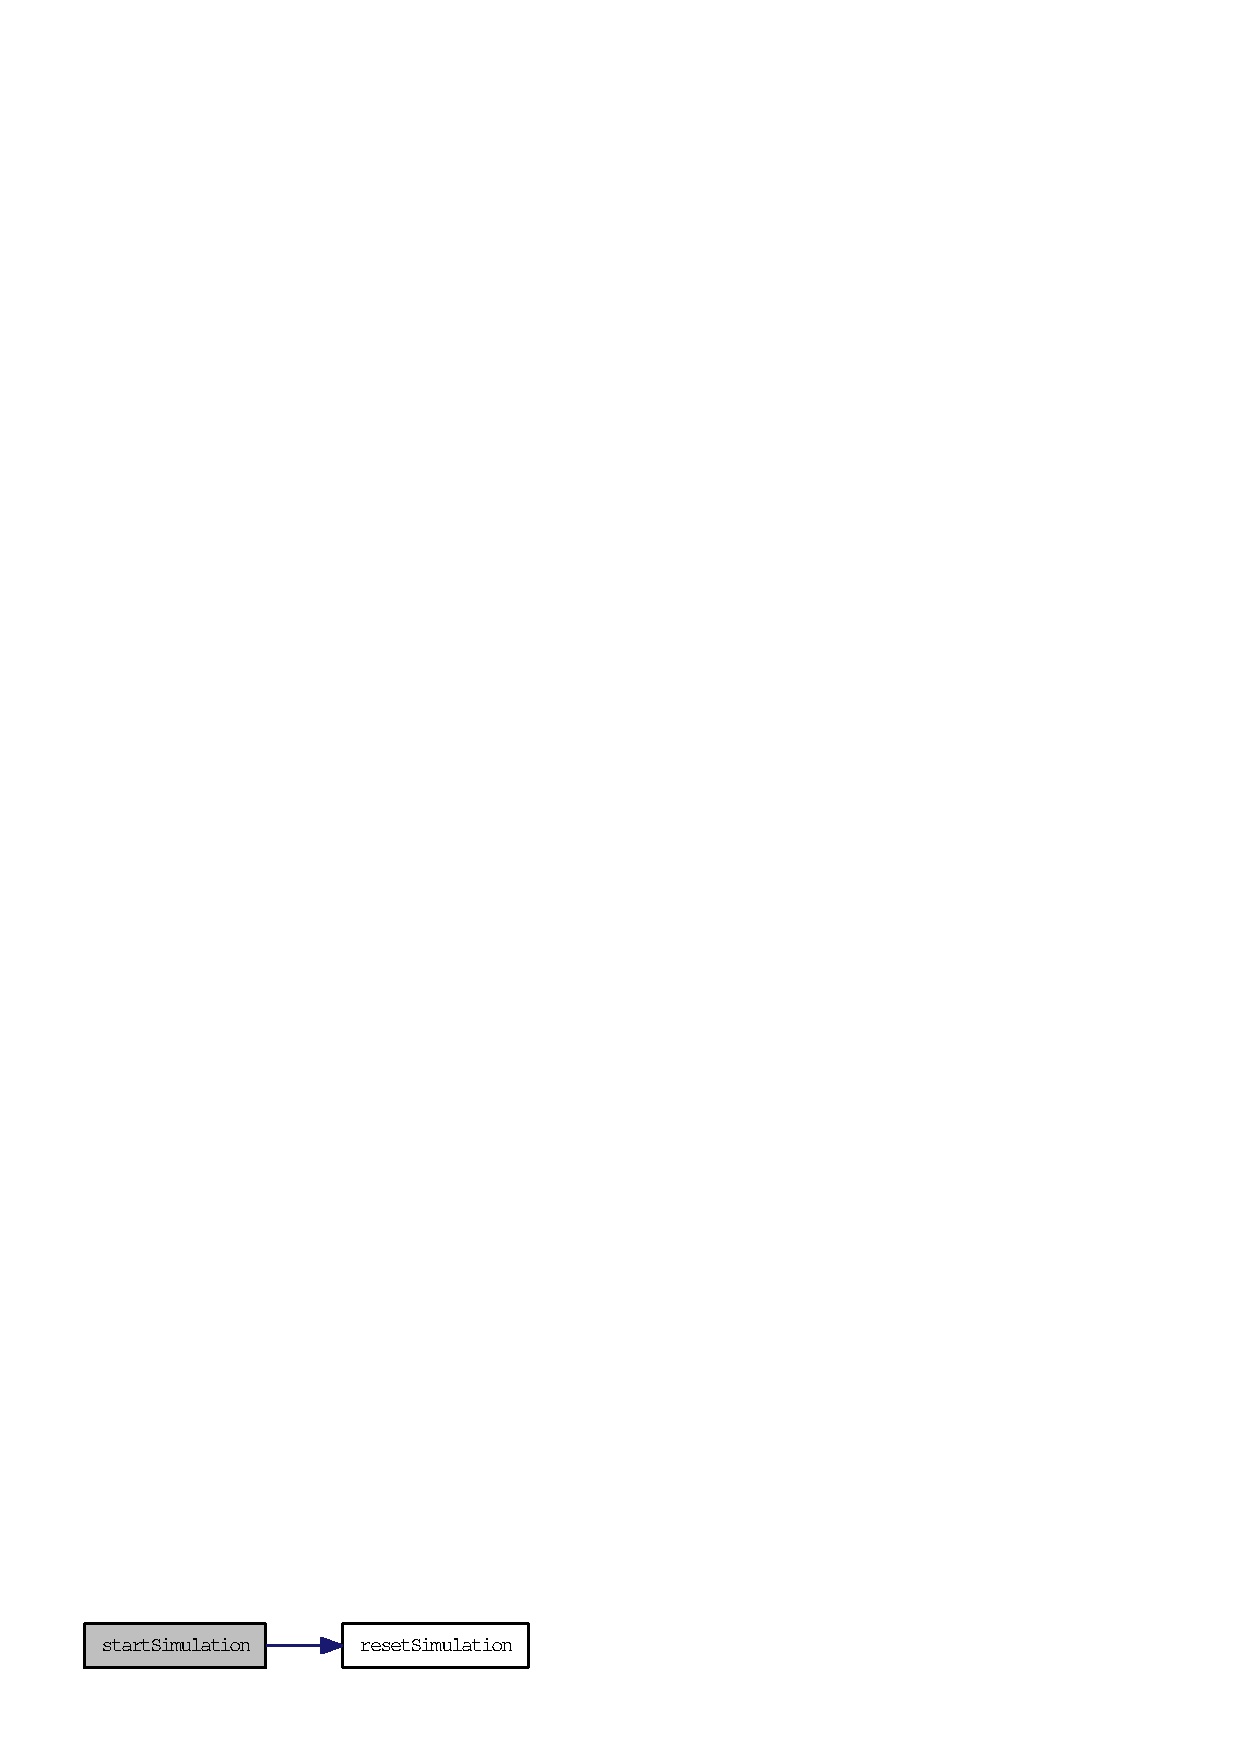
\includegraphics[width=129pt]{group__dcsc__msg__buffer__access_g0adb3aacb8d7ad32ceabe66a9dcbb401_cgraph}
\end{center}
\end{figure}
\hypertarget{group__dcsc__msg__buffer__access_gd871881385919aff64a8b679984cd018}{
\index{dcsc_msg_buffer_access@{dcsc\_\-msg\_\-buffer\_\-access}!stopSimulation@{stopSimulation}}
\index{stopSimulation@{stopSimulation}!dcsc_msg_buffer_access@{dcsc\_\-msg\_\-buffer\_\-access}}
\subsubsection[stopSimulation]{\setlength{\rightskip}{0pt plus 5cm}void stop\-Simulation ()}}
\label{group__dcsc__msg__buffer__access_gd871881385919aff64a8b679984cd018}


Stop the simulation. 

Cleanup function for the simulation feature. 

Definition at line 1800 of file dcsc\-Msg\-Buffer\-Interface.c.

Referenced by main(), and wait\-Condition().